
%%  本模板推荐以下方式编译:
%%     1. PDFLaTeX[推荐]
%%     2. xelatex [含中文推荐]
%%  注意:
%%  1. 文件默认的编码为 UTF-8 对于windows,请选用支持UTF-8编码的编辑器。
%%   2. 若是模板有什么问题,请及时与我们取得联系,Email:latexstudio@qq.com。
%%   3. 可以到  https://ask.latexstudio.net 提问
%%   4. 请安装 最新版本的 TeXLive 地址:
%%   http://mirrors.ctan.org/systems/texlive/Images/texlive.iso

\documentclass{apmcmthesis}

\usepackage{url}
\usepackage{longtable}
\usepackage{graphicx} 
\usepackage{subfigure} 
%%%%%%%%%%%%填写相关信息%%%%%%%%%%%%%%%%%%%%%%%%%%
\tihao{C}                            %选题
\baominghao{apmcm2306348}                 %参赛编号
\begin{document}

\pagestyle{frontmatterstyle}

\begin{abstract}


\end{abstract}
This paper, first and foremost, delves into the development trends of new energy electric vehicles by establishing multiple fitting models. We have also constructed predictive models to explore the future development of new energy electric vehicles. Finally, we established a lifecycle model to investigate the impact of new energy electric vehicles on the environment.

For the first question, we began by preprocessing the data, addressing missing values and outliers, and visualizing the data. Subsequently, we initially explored the factors influencing the development of new energy electric vehicles using \textbf{Pearson correlation analysis}. Following that, we employed the \textbf{Grey Relational Analysis method} to further investigate the primary factors. The key factors identified include policy, economic, environmental, infrastructure, and energy factors. Finally, we established a \textbf{multiple linear regression model} based on these five key factors to further explore their impact on the development of new energy electric vehicles in China.

For the second question, we collected data on the production and sales of new energy electric vehicles from January 2017 to September 2023. Since the data has a time series nature, we utilized two time series models, \textbf{LSTM} and \textbf{ARIMA}, to predict the future 10 years of development trends for new energy electric vehicles in China. We found that over the next 10 years, China's new energy electric vehicles will continue to develop rapidly, with an increasing growth rate in production and sales.

For the third question, we collected global production and sales data of traditional and new energy vehicles from 2018 to 2022. To explore the relationship between the two, we established a \textbf{linear double logarithmic regression model}. We found that the development of traditional vehicles is related to new energy electric vehicles in a power function. As new energy electric vehicles develop, the growth of traditional vehicles will gradually slow down, eventually stabilizing.

For the fourth question, we collected policies from foreign countries that resisted the development of China's new energy electric vehicles. Subsequently, using the \textbf{Grey Forecasting Model}, we predicted the development trend of China's new energy vehicles without these policies and compared it with actual data. The results indicate that, even in the face of foreign policy restrictions, China's export volume of new energy vehicles is expected to increase year by year, with a potential breakthrough of 2.7 million units in 2024.

For the fifth question, to quantify the impact of new energy electric vehicles on the ecological environment, we conducted a \textbf{Life Cycle Assessment (LCA)}, focusing on exploring the contribution of electric buses to carbon reduction. The results show that, under the assumption of a city population of 1 million, electric buses can achieve a carbon reduction of \textbf{275.75 tons}, with a reduction rate of \textbf{21.428\%}. This indicates that new energy electric vehicles have significantly improved the ecological environment in urban electrification.

\keywords{New energy electric vehicle \quad Grey Relation Analysis \quad  multiple linear regression\quad LSTM \quad ARIMA \quad linear double logarithmic regression \quad Grey prediction \quad LCA  }

\newpage
%目录
\tableofcontents


\newpage
\pagestyle{mainmatterstyle}
\setcounter{page}{1}
\section{Introduction}
\subsection{Background}
In recent years, with the emergence of a new round of technological revolution and industrial transformation, the new energy vehicle industry has entered a phase of accelerated development. China's new energy vehicle industry, after years of continuous efforts, has seen a significant improvement in technological levels, a progressively perfected industrial system, and a substantial enhancement in the competitiveness of enterprises. It is presenting a favorable situation of "dual improvement" in market size and development quality. Since 2011, the Chinese government has actively promoted the development of new energy electric vehicles and has formulated a series of preferential policies.

This article will utilize various data related to China's new energy vehicles to explore the development situation and future expectations of China's new energy vehicle industry. It aims to promote the multiple benefits and contributions of new energy electric vehicles.
\subsection{Restratment of Problems}

\begin{itemize}
    \item[*] Analyze the main factors influencing the development of new energy electric vehicles in China based on data, and discuss the impact of these factors on the development of new energy electric vehicles in China.
    \item[*] Establish a mathematical model to describe and predict the development trends of new energy vehicles in China for the next ten years.
    \item[*]  Analyze the impact of new energy vehicles on the global traditional energy vehicle industry.
    \item[*] Analyze the impact of foreign policies resisting the development of new energy vehicles in China on the development of new energy electric vehicles in China.
    \item[*] Analyze the impact of new energy vehicles on the ecological environment based on assumptions and write an open letter to citizens, promoting the benefits of new energy electric vehicles and the contributions of the electric vehicle industry.
    \end{itemize}

\subsection{Models}
For question one, based on the collected data, we employed the Grey Relational Analysis method to analyze the primary factors influencing the sales of new energy electric vehicles in China. Subsequently, we established a multiple linear regression model based on these key factors to explore their impact on the development of new energy electric vehicles in China.

Regarding question two, using the collected data, we utilized two time series models, namely LSTM and ARIMA, to predict the development trends of new energy electric vehicles in China over the next ten years.

Concerning question three, we constructed an exponential fitting model to explore the impact of new energy electric vehicles on the global traditional energy vehicle industry.

For question four, due to limited data, we employed the Grey Prediction model. We compared the predicted results with the actual outcomes and analyzed the impact of resistance policies on the development of new energy electric vehicles.

As for question five, we utilized the Life Cycle Assessment method to analyze the carbon emissions of diesel buses and electric buses throughout their lifecycle, quantifying the impact of new energy electric vehicles on the ecological environment.
\section{Data Description} 

\begin{longtable}{c c c c}
Data & Source  \\ \hline 
Production of new energy vehicles  & China AutoParts Industry Association   \\
Output of power batteries &  China Industry Technology Innovation Strategic Alliance For Electric Vehicle \\
Exports of new energy vehicles & Chinese general administration \\
Number of public charging piles & The State Council of the People's Republic of China \\
BeijingAQI & China National Environmental Monitoring Centre \\
Consumer Price Index & National Bureau of Statistics \\
Environmental awareness & National Bureau of Statistics \\
International energy market prices & National Bureau of Statistics \\
Power generation & National Bureau of Statistics \\ 
Global automobile production & International Organization of Motor Vehicle Manufacturers \\ \hline
\end{longtable}


\section{Symbols and Assumptions}
\subsection{Symbol Description}
\begin{table}[h]
    \centering
    \begin{tabular}{cc}
    \hline
    sign        & Instructions                      \\ \hline
    $\beta_i$   & regression coefficient            \\
    $X_i$       & Main factor      \\
    Y           & Production of Electric Vehicles    \\
    $\varepsilon$ & error                             \\
    $P_{xy}$     & Pearson's correlation coefficient \\
    T           & temperature                       \\ \hline
    \end{tabular}
    \end{table}

\subsection{Assumptions}
We assume that the data sources are reliable
\section{Models and Solutions}

\subsection{Question1}
\paragraph{Data Pre-processing}
We initiated the data cleaning process by conducting missing value and outlier detection, and the results are illustrated in Figure 1,2. Due to the time-series nature of the data, we addressed missing values by filling them with the average of the adjacent two values. For outlier values, we undertook the collection of the anomalous data anew.
\begin{figure}[htbp]
    \centering
    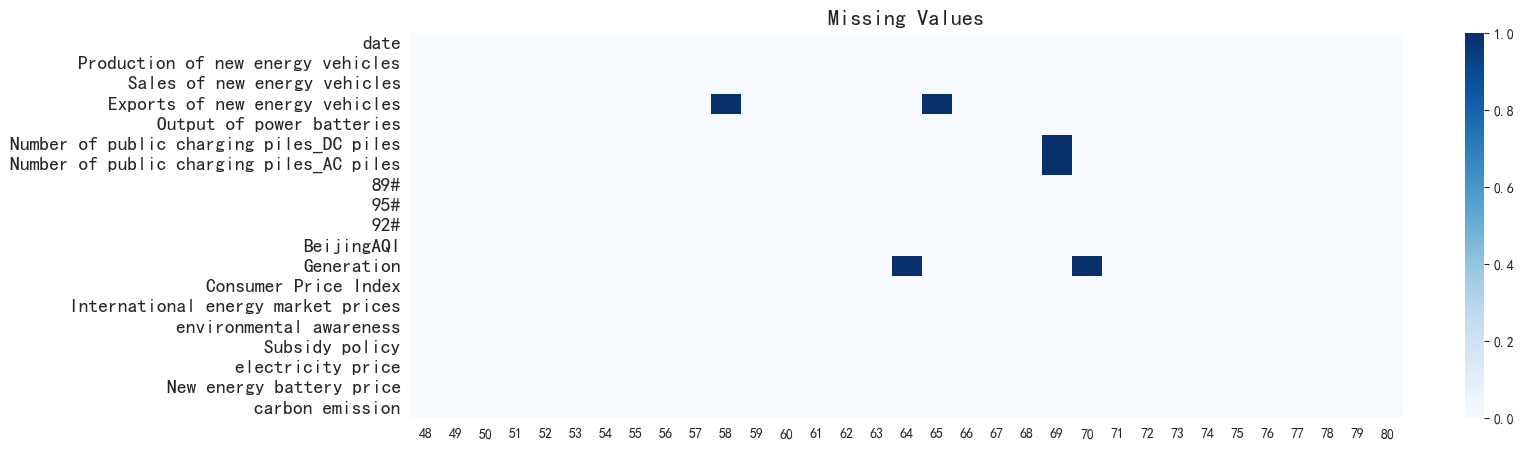
\includegraphics[scale=0.4]{figures/Figure/问题一/数据预处理/Missing Values.png}
    \caption{Missing Values}
\end{figure}

\begin{figure}[htbp]
    \centering
    \subfigure[1]{
    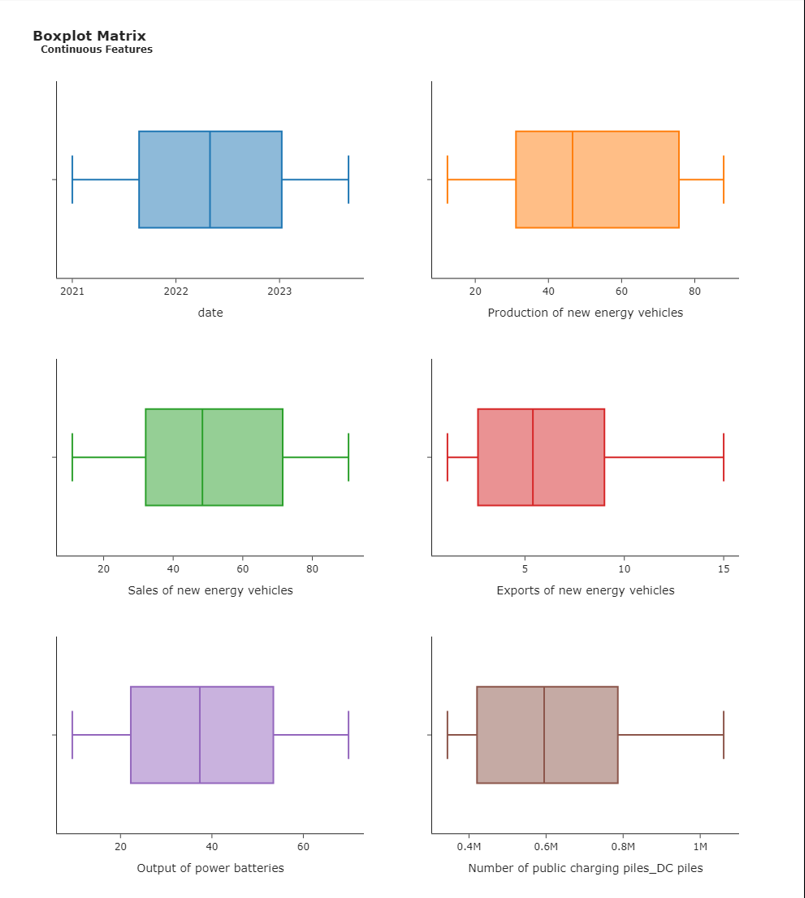
\includegraphics[scale=0.4]{figures/Figure/问题一/数据预处理/box2.png} \label{1}
    }
    \quad
    \subfigure[2]{
    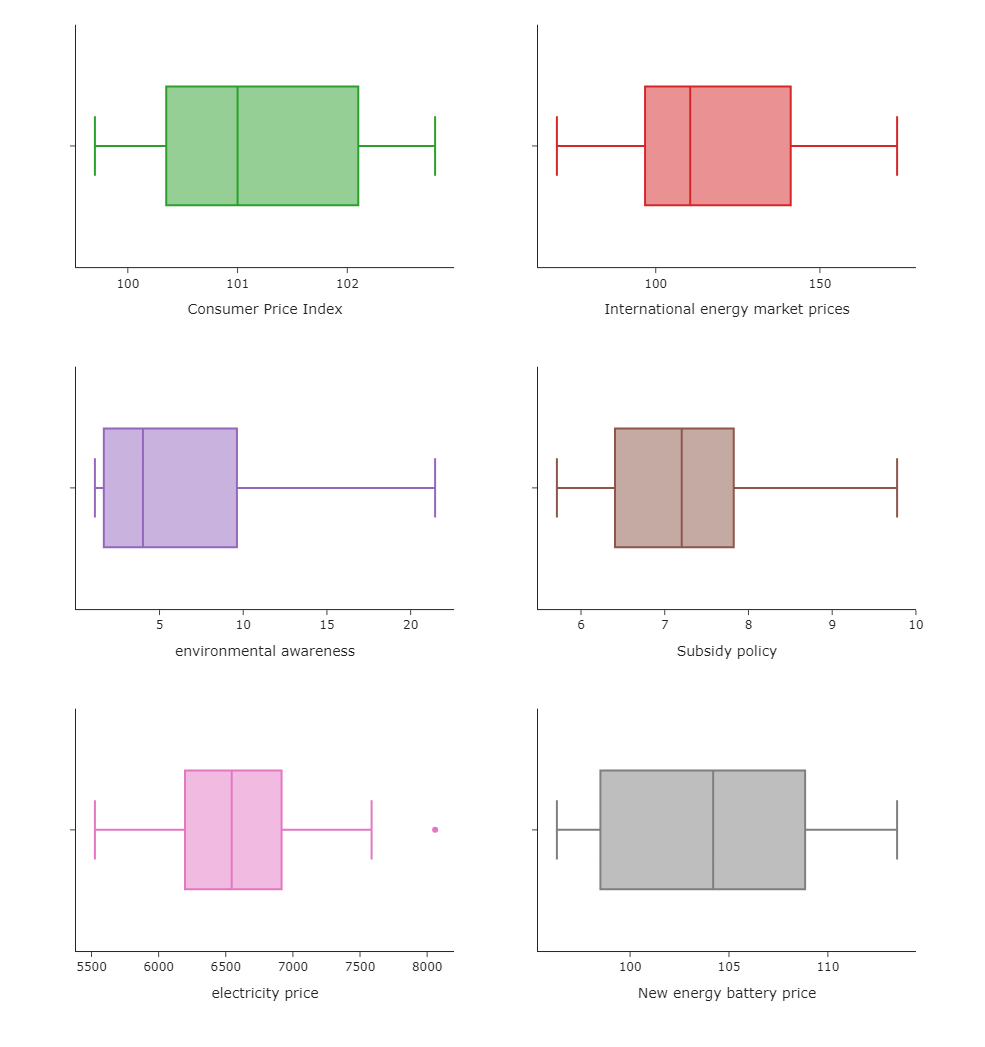
\includegraphics[scale=0.35]{figures/Figure/问题一/数据预处理/box3.png} \label{2} 
    }
    \caption{Boxplot Matrix}
    \end{figure}

Figure 3 represents the descriptive analysis of our data.
We initially employed Pearson correlation analysis, calculating the correlation coefficients for each feature to preliminarily observe the key factors influencing the sales of new energy vehicles. 
\begin{figure}[htbp]
    \centering
    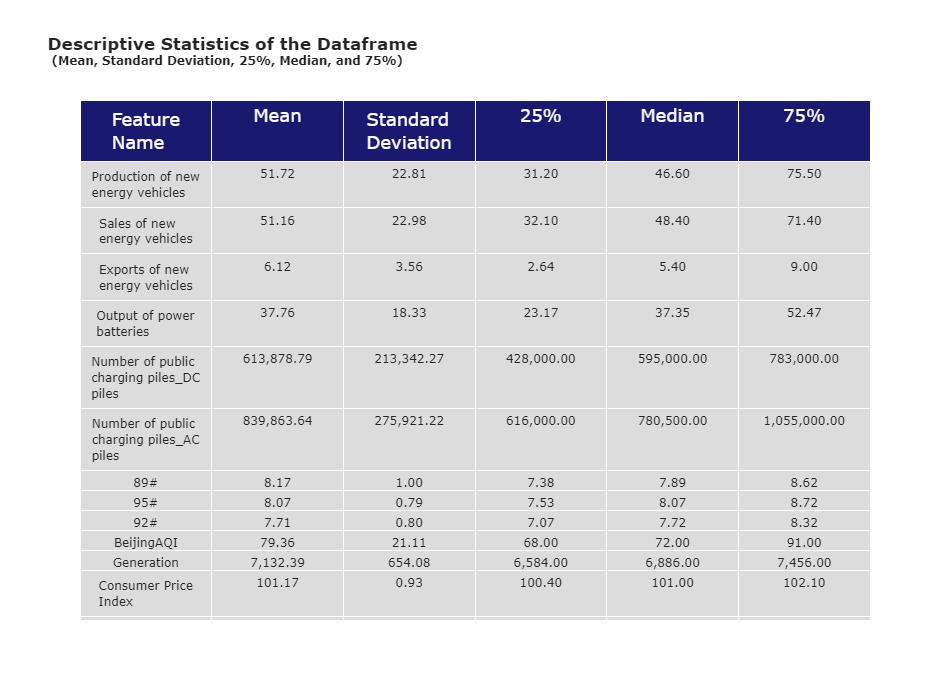
\includegraphics[scale=0.3]{figures/Figure/问题一/数据预处理/description.png}
    \caption{Data description}
\end{figure}

\begin{figure}[htbp]
    \centering
    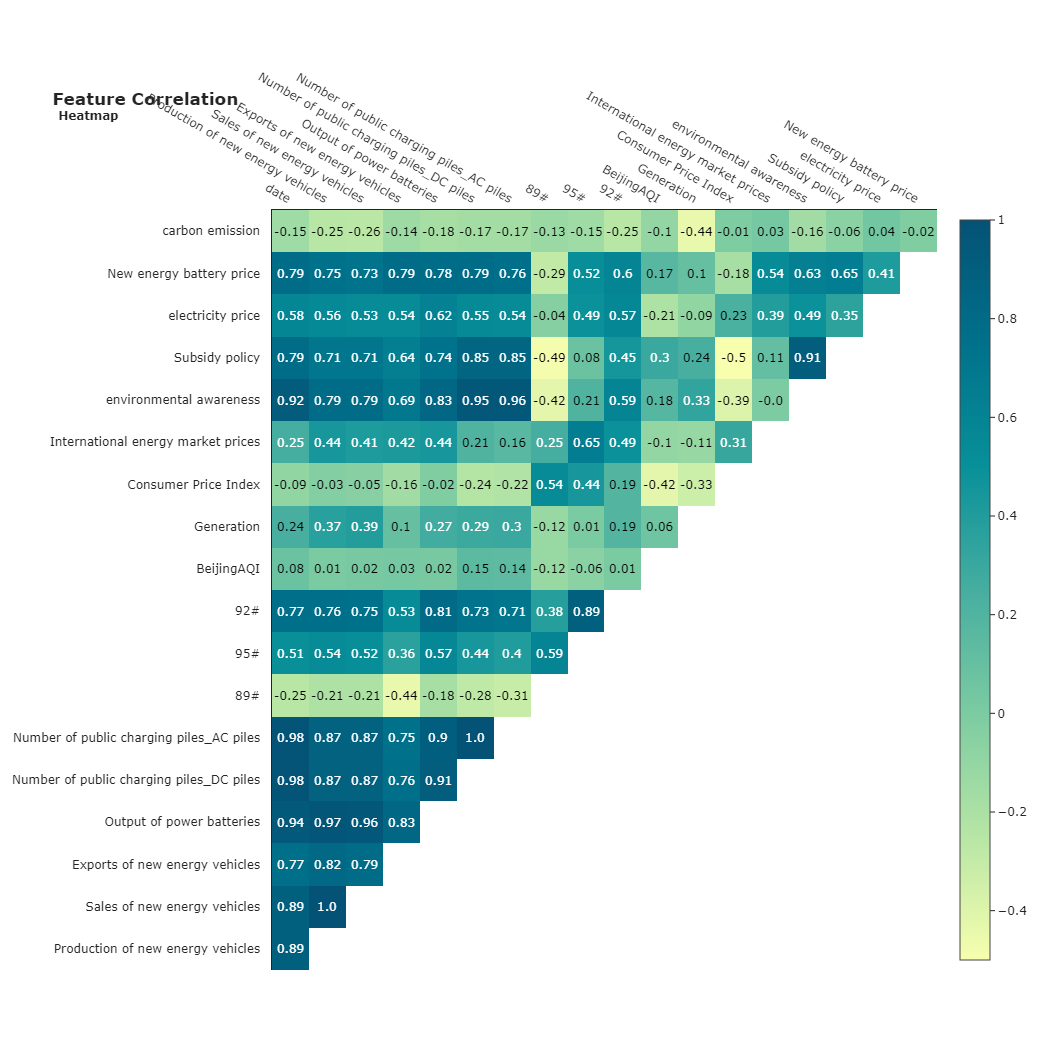
\includegraphics[scale=0.35]{figures/Figure/问题一/数据预处理/Correlation Heap.png}
    \caption{Correlation Heap}
\end{figure}

\newpage

We first utilized Pearson correlation analysis, calculating the correlation coefficients for each feature to preliminarily observe the key factors influencing the sales of new energy vehicles. The correlation coefficient heatmap is shown in Figure 4.

Through the heatmap, we identified factors highly correlated with the production of new energy vehicles, including the price of new energy batteries, government subsidies, environmental awareness, the number of charging stations, and the production of power batteries. The correlation coefficients (P) for these factors are 0.75, 0.71, 0.79, 0.87, and 0.97, respectively.

\paragraph{Grey Relation Analysis}

\begin{figure}[h]
    \centering
    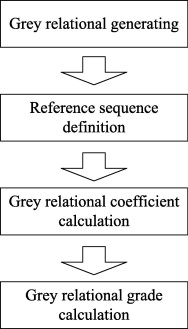
\includegraphics[scale=1]{figures/Figure/Grey Relation Analysis.jpg}
    \caption{GRA Framework}
\end{figure}
Then, we further analyzed the main factors influencing new energy vehicle production using the Grey Relational Analysis method. The process of Grey Relational Analysis is illustrated in Figure 5.
Firstly, we took the new energy production from January 2017 to September 2023 as the reference sequence and treated other feature data as sub-sequences. We initially normalized the data to eliminate the influence of different scales, using the formula $(X-Min)/(Max-Min)$. Subsequently, we calculated the degree of correlation between each element in the processed sub-sequence and the corresponding element in the reference sequence.
Let the reference sequence be denoted as \(x_0=\{x_0(1),x_0(2), \cdots, x_0(n)\}\), and the sub-sequence as \(x_i=\{x_i(1),x_i(2), \cdots, x_i(n)\}\). We computed the minimum difference between the reference sequence and the sub-sequence, denoted as \(a = \min|x_0(k)-x_i(k)|, \forall i,k\). We defined \(\gamma(x_0(k),x_i(k))=\frac{a+\rho b}{|x_0(k)-x_i(k)|+\rho b}\), where \(\rho\) is the resolution coefficient, set to 0.5. Afterward, we calculated the degree of correlation for each sequence, defined as \(\gamma(x_0,x_i)=\frac{\sum_{k=1}^n \gamma(x_0(k),x_i(k))}{n}\), representing the correlation of a specific indicator with the overall system. The results are shown in Table 1.
\begin{longtable}{ccc}
    \hline
    Evaluation item                           & Grey relational degree & Ranking \\ \hline
    Output of power batteries                 & 0.895                  & 1       \\
    Number of public charging piles		      & 0.859                  & 2       \\
    International energy market prices        & 0.749                  & 3       \\
    Subsidy policy                            & 0.746                  & 4       \\
    BeijingAQI                                & 0.734                  & 5       \\
    New energy battery price                  & 0.719                  & 6       \\
    Generation                                & 0.716                  & 7      \\
    electricity price                         & 0.715                  & 8      \\
    Consumer Price Index                      & 0.696                  & 9      \\
    89\#                                      & 0.685                  & 10      \\
    environmental awareness                   & 0.647                  & 11      \\
    carbon emission                           & 0.622                  & 12     
\end{longtable}
Combining the results of Pearson correlation analysis and Grey Relational Analysis, we find that the main factors influencing the development of new energy electric vehicles can be categorized into five major factors: policy factors, economic factors, charging infrastructure factors, environmental factors, and energy factors.

\paragraph{Multiple linear regression model}
We use the earlier conclusion, namely the five major factors influencing the development of new energy electric vehicles, to establish a multiple linear regression model to further explore the impact of these factors on the development of new energy electric vehicles. The model can be expressed as:

\[ Y = \beta_0 + \beta_1X_1 + \beta_2X_2 + \beta_3X_3 + \beta_4X_4 + \beta_5X_5 + \varepsilon \]

where,
\( Y \) represents the production of new energy electric vehicles,
\( X_1 \) represents policy factors,
\( X_2 \) represents economic factors,
\( X_3 \) represents infrastructure factors,
\( X_4 \) represents environmental factors,
\( X_5 \) represents energy factors,
\( \beta_0 \) is the intercept,
\( \beta_1, \beta_2, \beta_3, \beta_4, \beta_5 \) are the regression coefficients for each factor,
\( \varepsilon \) is the error term.

The goal of the least squares method is to minimize the sum of squared differences between the actual values \( Y \) and the estimated values \( \hat{Y} \). In this problem, the sample regression function is given by:

\[ Y = \beta_0 + \beta_1X_1 + \beta_2X_2 + \beta_3X_3 + \beta_4X_4 + \beta_5X_5 + \varepsilon \]

For the \( i \)-th sample, the difference between the actual and estimated values is:

\[ e_i = Y - \hat{Y} = Y - (\beta_0 + \sum_{i=1}^{5}\beta_iX_i) \]

The sum of squared residuals for all \( i \) (with a sample size of \( n \)) is:

\[ Q = \sum_{i=1}^ne_i^2 = \sum_{i=1}^{n}[ Y - (\beta_0 + \sum_{i=1}^{5}\beta_iX_i)]^2 \]

Let \( R_{ji} \) denote the residuals of the \( j \)-th explanatory variable \( X_j \) after regressing on other explanatory variables using the Ordinary Least Squares (OLS) method:

\[ \beta_j = \frac{\sum_{i=1}^{n}R_{ji}Y}{\sum_{i=1}^{n}R_{ji}^2} \]

The model calculation results are given by \( Y = 0.7785X_1 + 3.091X_2 + 1.200X_3 + 0.001X_4 + 0.207X_5 \). The R-squared value is 0.991, and the p-value from the F-test is 1.29e-27, indicating that the regression model is statistically significant. The fitted plot is shown in Figure 6.
\begin{figure}[h]
    \centering
    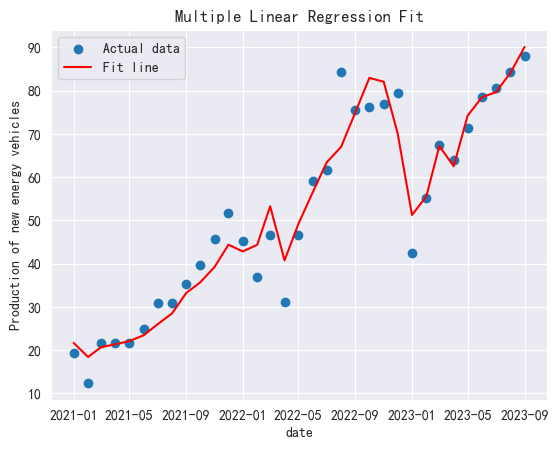
\includegraphics[scale=1]{figures/Figure/问题一/Regession Fit.png}
    \caption{Regession Fit}
\end{figure}

\subsection{Question2}
We collected data on new energy production, sales, and export quantities from January 2017 to September 2023, totaling 84 data points. Initially, we established LSTM and ARIMA time series models, conducted training, and selected the optimal model based on the fitting performance to serve as the main model for predicting the development trend. Finally, we analyzed the future development trends of China's new energy electric vehicles based on the forecasting results.

\paragraph{LSTM}
Long Short-Term Memory (LSTM) is a specialized structure proposed to overcome the gradient explosion or vanishing problems associated with Recurrent Neural Networks (RNNs). It is capable of retaining information for a long duration, allowing it to not only extract information from individual data points but also from entire data sequences. LSTM is primarily composed of three gates: the forget gate, input gate, and output gate.\cite{LSTM}

\begin{figure}[h]
    \centering
    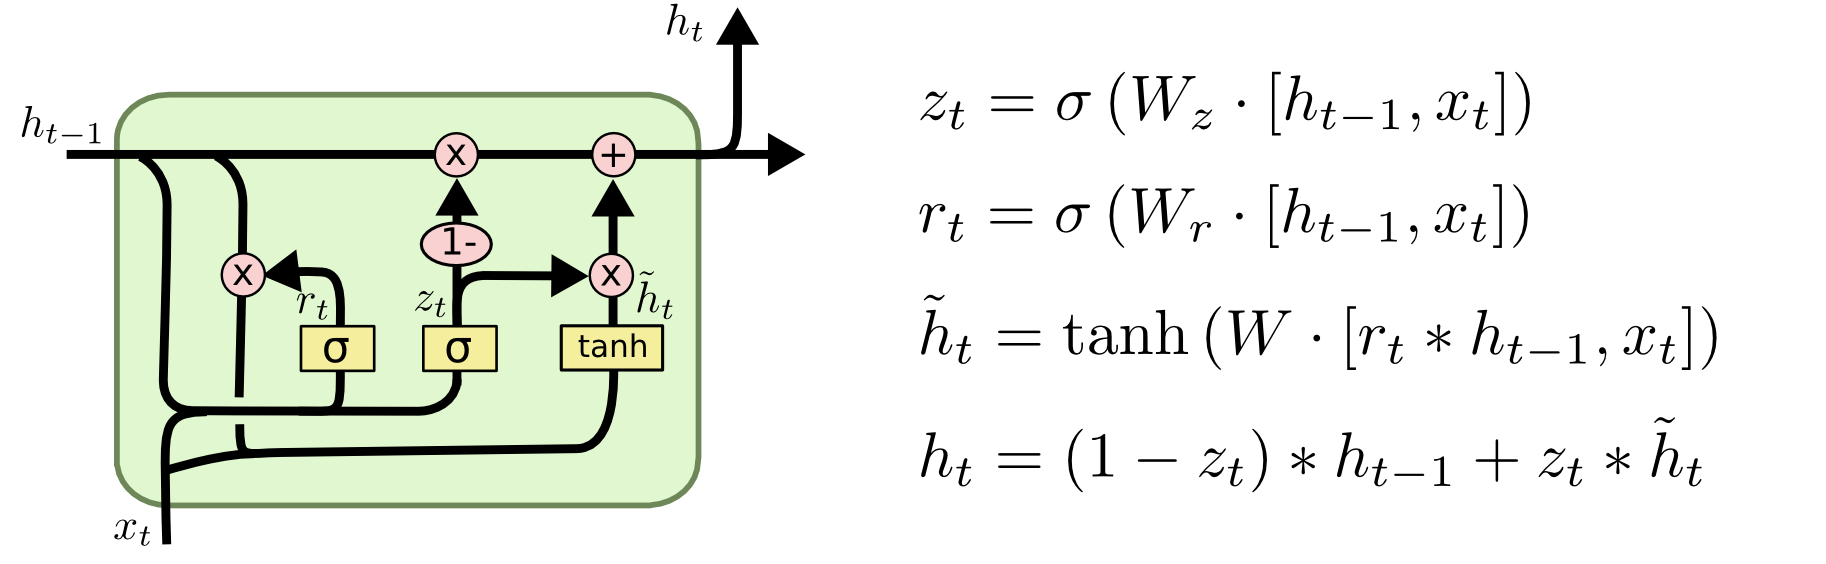
\includegraphics[scale=0.6]{figures/Figure/LSTM Framework.png}
    \caption{LSTM Framework}
\end{figure}

The core concepts of LSTM lie in the cell state and gate structures. The cell state serves as the path for information transmission, while the gate structures facilitate the addition and removal of information\cite{LSTM}, controlled by sigmoid activation functions. The input gate \( i_t \) regulates how much information from the candidate state \( c_t \) at the current time step needs to be stored. The forget gate \( f_t \) controls how much information from the internal state \( c_{t-1} \) at the previous time step should be forgotten. The output gate \( o_t \) manages how much information from the current internal state \( c_t \) needs to be output to the external state \( h_t \). The formulas for calculating the three gates are as follows:

\begin{equation}
    \begin{aligned}
        i_t & = \sigma(W_i x_t + U_i h_{t-1} + b_i) \\
        f_t & = \sigma(W_f x_t + U_f h_{t-1} + b_f) \\
        o_t & = \sigma(W_o x_t + U_o h_{t-1} + b_o) \\
        c_t & = f_t \odot c_{t-1} + i_t \odot \tanh(W_c x_t + U_c h_{t-1} + b_c) \\
        h_t & = o_t \odot \tanh(c_t)
    \end{aligned}
\end{equation}
    

Here, \(\sigma\) represents the sigmoid activation function, \(\odot\) denotes element-wise multiplication, and \(\tanh\) is the hyperbolic tangent function. The parameters \(W_i, U_i, b_i, W_f, U_f, b_f, W_o, U_o, b_o, W_c, U_c, b_c\) are weight matrices and bias vectors specific to each gate.

We use TensorFlow to construct an LSTM model. We use collected data related to new energy electric vehicles as input feature vectors. Considering that LSTM can learn temporal features from data, reduce model training time, and mitigate overfitting risks, our LSTM employs a network structure with 4 layers, each containing 60 neurons. We use mean squared error as the loss function and set the learning rate to 0.01.
Results are in Figure8,9
\begin{figure}[h]
    \centering
    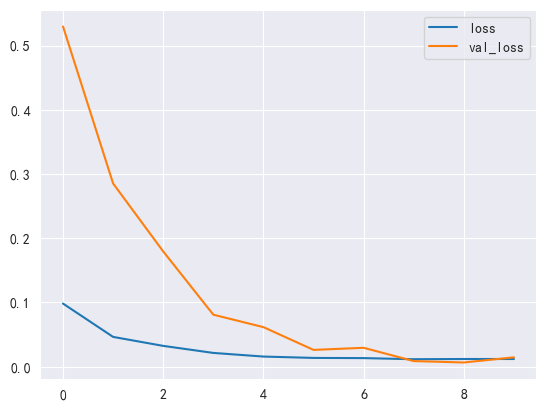
\includegraphics[scale=0.5]{figures/Figure/loss.png}
    \caption{Loss}
\end{figure}

\begin{figure}[h]
    \centering
    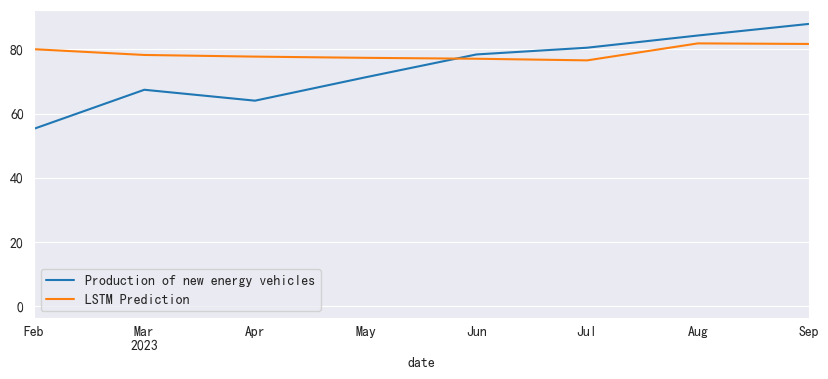
\includegraphics[scale=0.5]{figures/Figure/fitting.png}
    \caption{LSTM Fitting}
\end{figure}


\paragraph{ARIMA}
Autoregressive Integrated Moving Average (ARIMA) is a commonly used local statistical method for time series forecasting. ARIMA captures the standard temporal structures (patterned time organization) within the input dataset. The ARIMA algorithm is particularly useful for datasets that can be mapped to stationary time series.\cite{ARIMA}
\begin{figure}[h]
    \centering
    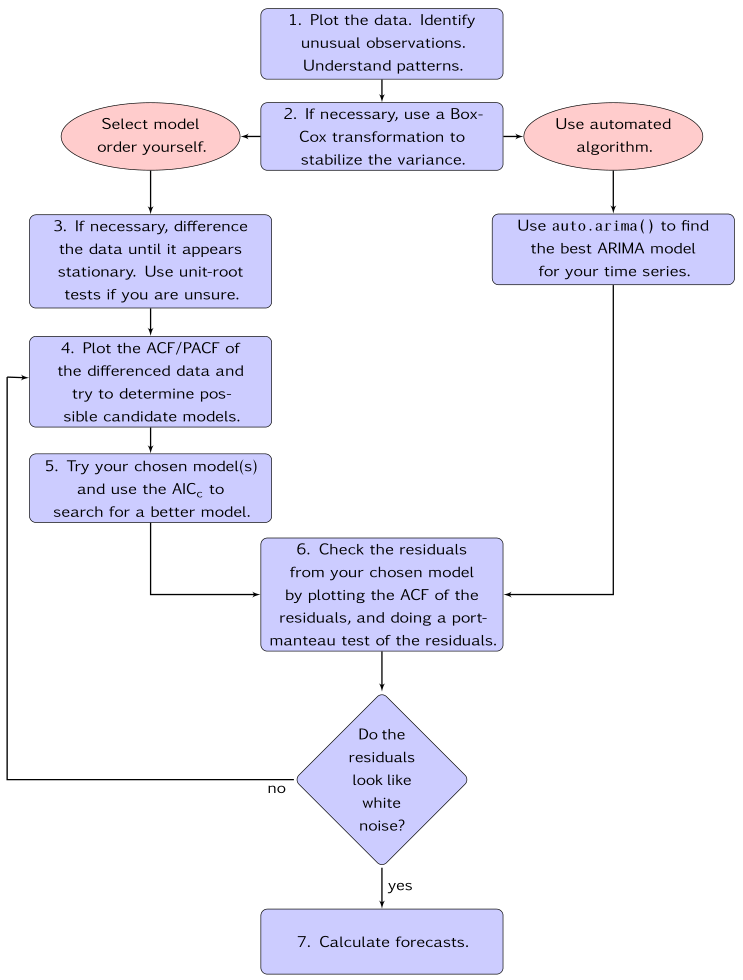
\includegraphics[scale=0.3]{figures/Figure/arimaflowchart.png}
    \caption{ARIMA Framework}
\end{figure}

We first conduct seasonal trend decomposition to observe the characteristics of the time series. The results are shown in Figure 11. We can observe a significant increase in new energy production and sales during the period of November to December each year, indicating a seasonal pattern. I also noticed that, starting from 2021, the development of China's new energy vehicle industry has been rapid. Due to the presence of seasonal features, we incorporate a seasonal cycle of 12 into the ARIMA model.
\begin{figure}[htbp]
    \centering
    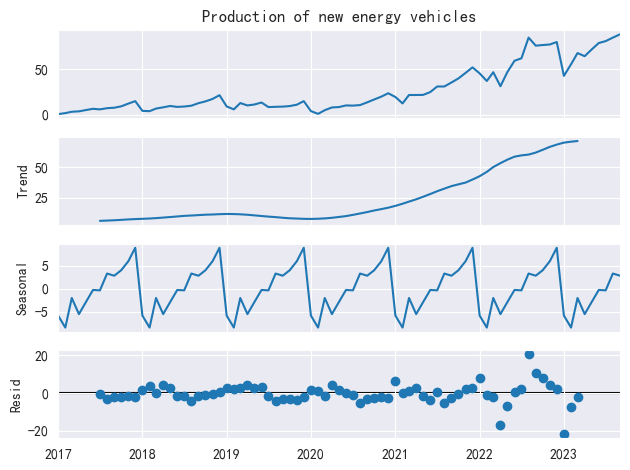
\includegraphics[scale=0.8]{figures/Figure/seasonal_decompose.png}
    \caption{Seasonal trend decompostion}
\end{figure}
To meet the modeling conditions of ARIMA, preprocessing of the demand time series is required, and a differencing operation is applied to obtain a stationary time series. The basic form of the ARIMA(p, I, q) model is as follows:

\[ x_t = \phi_0 + \phi_1 x_{t-1} + \ldots + \phi_p x_{t-p} + \epsilon_t - \theta_1 \epsilon_{t-1} - \ldots - \theta_q \epsilon_{t-q} \]

Here, \( \{x_t\} \) is the stationary time series, \( \{\epsilon\} \) is a mutually independent white noise sequence, \( \{\phi_i\} \) (for \(i = 1, 2, \ldots, p\)) and \( \{\theta_j\} \) (for \(j = 1, 2, \ldots, q\)) are the model parameters to be estimated, \(p\) is the autoregressive order, and \(q\) is the moving average order.

The data series is differenced progressively, with the first-order difference represented as:

\[ \nabla x_t = x_t - x_{t-1} = (1 - B)x_t \]

Here, \(\nabla\) is the differencing operator, \(B\) is the lag operator, and \(Bx_t = x_{t-1}\).

The \(d\)-th order difference is expressed as:

\[ \nabla^d x_t = (1 - B)^d x_t = \sum_{i=0}^{d} (-1)^i \binom{d}{i} x_{t-i} \]

After \(d\)-th order differencing, (6.2) is represented as:

\[ \Phi(B) \nabla^d x_t = \Theta(B) \epsilon_t \]

Here, \(\Phi(B) = 1 - \phi_1 B - \ldots - \phi_p B^p\) is the autoregressive coefficient polynomial of the stationary and invertible ARIMA(p, I, q) model.

After undergoing two differencing operations (i.e., \(d = 2\)), the data becomes stationary. Subsequently, we determine the values of \(p\) and \(q\) through autocorrelation and partial autocorrelation plots,\(p\)=2,\(q\)=7, as illustrated in Figure 12.

\begin{figure}[htbp]
    \centering
    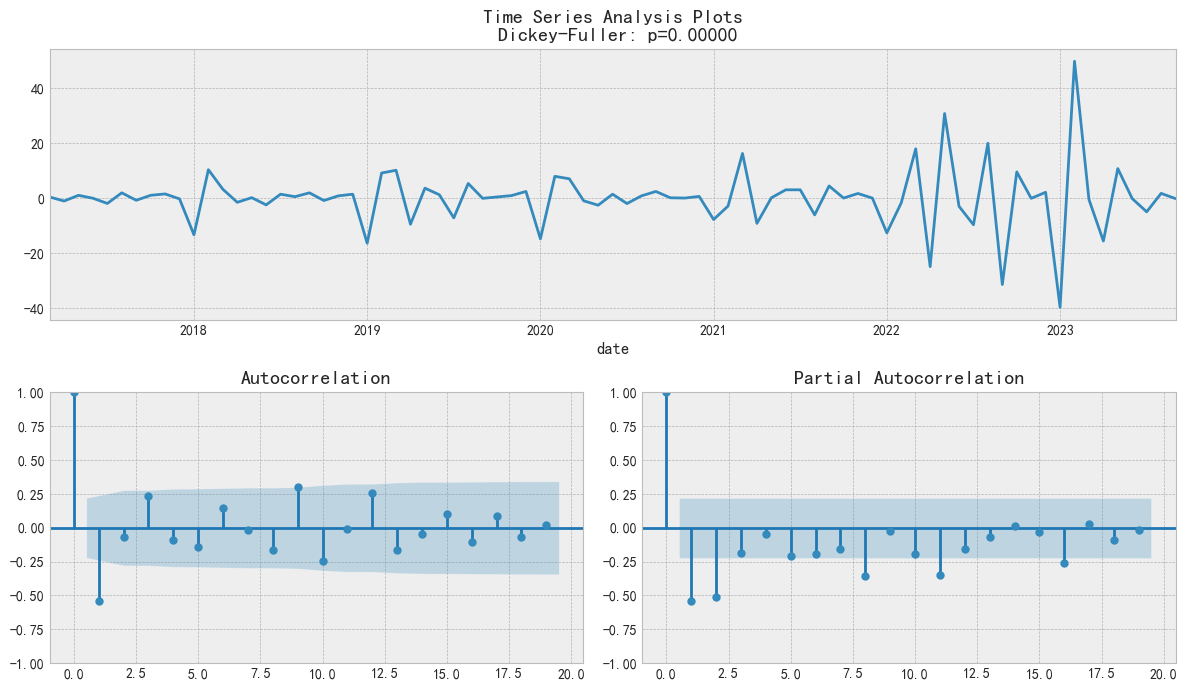
\includegraphics[scale=0.5]{figures/Figure/pd.png}
    \caption{}
\end{figure}

The fitting image of the ARIMA model is shown in Figure 13. Through comprehensive comparison, and considering the relatively small dataset, we choose the ARIMA model to forecast the future development trend of new energy electric vehicles in China over the next decade. Detailed predictions for the development of new energy electric vehicles in China over the next ten years can be found in Appendix Two.
\begin{figure}[htbp]
    \centering
    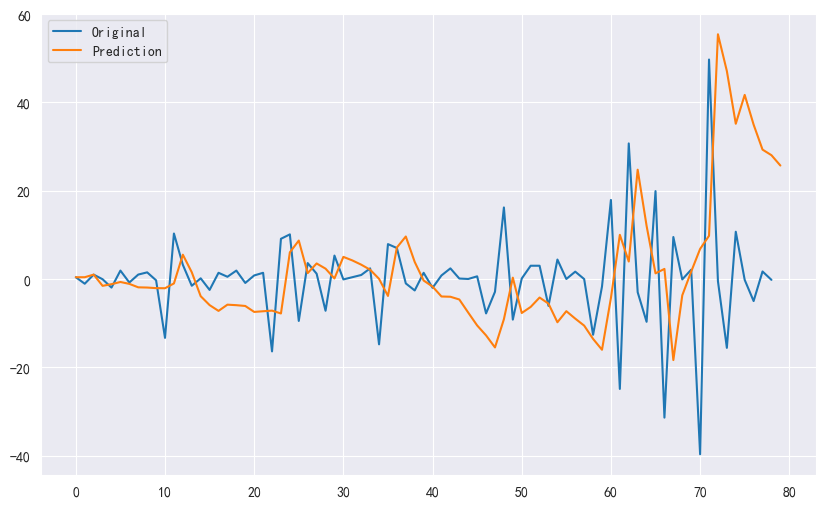
\includegraphics[scale=0.5]{figures/Figure/问题二/ARIMA fitting.png}
    \caption{ARIMA fitting}
\end{figure}

\begin{figure}[htbp]
    \centering
    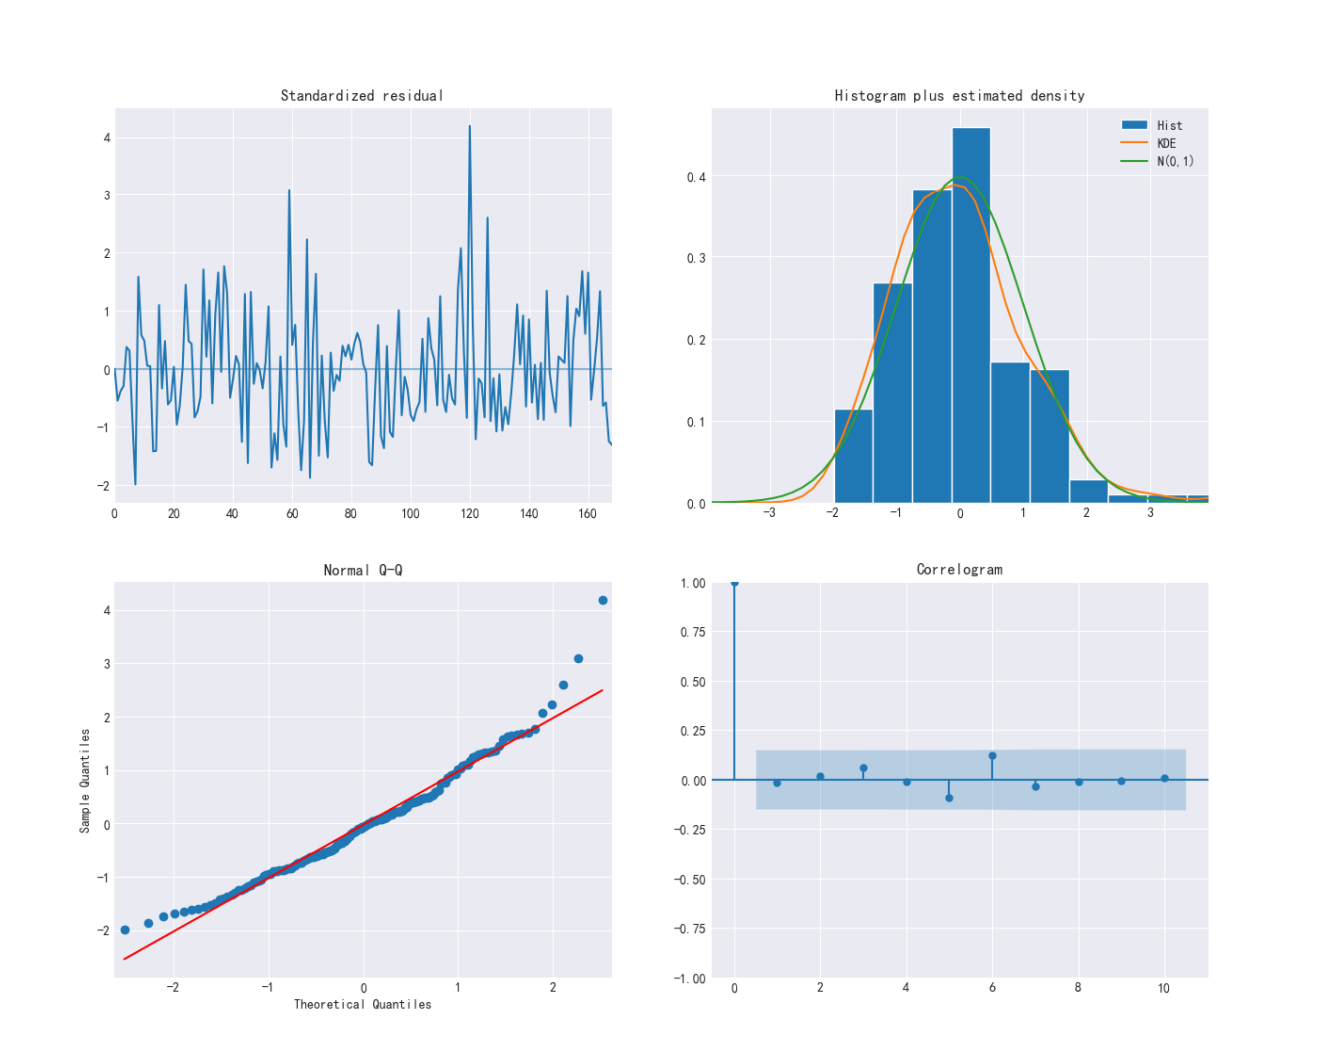
\includegraphics[scale=0.5]{figures/Figure/1234.png}
    \caption{Residual detection plot}
\end{figure}

From Figure 14 We find: In the upper right plot, we observe that the red KDE line closely follows the N(0,1) line (where N(0,1) is the standard representation of a normal distribution with mean 0 and standard deviation 1). This strongly indicates that the residuals are normally distributed. The qq plot in the lower left corner shows that the ordered distribution of residuals (blue dots) follows a linear trend obtained from a sample with a standard normal distribution N(0,1). Similarly, this indicates that the residuals are normally distributed. The upper left plot suggests that over time, the residuals do not exhibit significant seasonal changes and appear to be white noise. The lower right autocorrelation (ACF) plot further confirms this, showing low correlation between the time series residuals and their lagged values.

Observing the data, we find that the sales of new energy electric vehicles in China are on an upward trend over the next ten years, and the growth rate is increasing. Infrastructure and export volume are also expected to increase year by year.


\subsection{Question3}

With the development of new energy electric vehicles, the traditional automotive industry is inevitably constrained, either facing a decrease in sales or a slow growth. Analyzing based on sales as an indicator, we collected data and created scatter plots for the annual production and sales of both new energy and traditional energy vehicles, as shown below.

\begin{figure}[htbp]
    \centering
    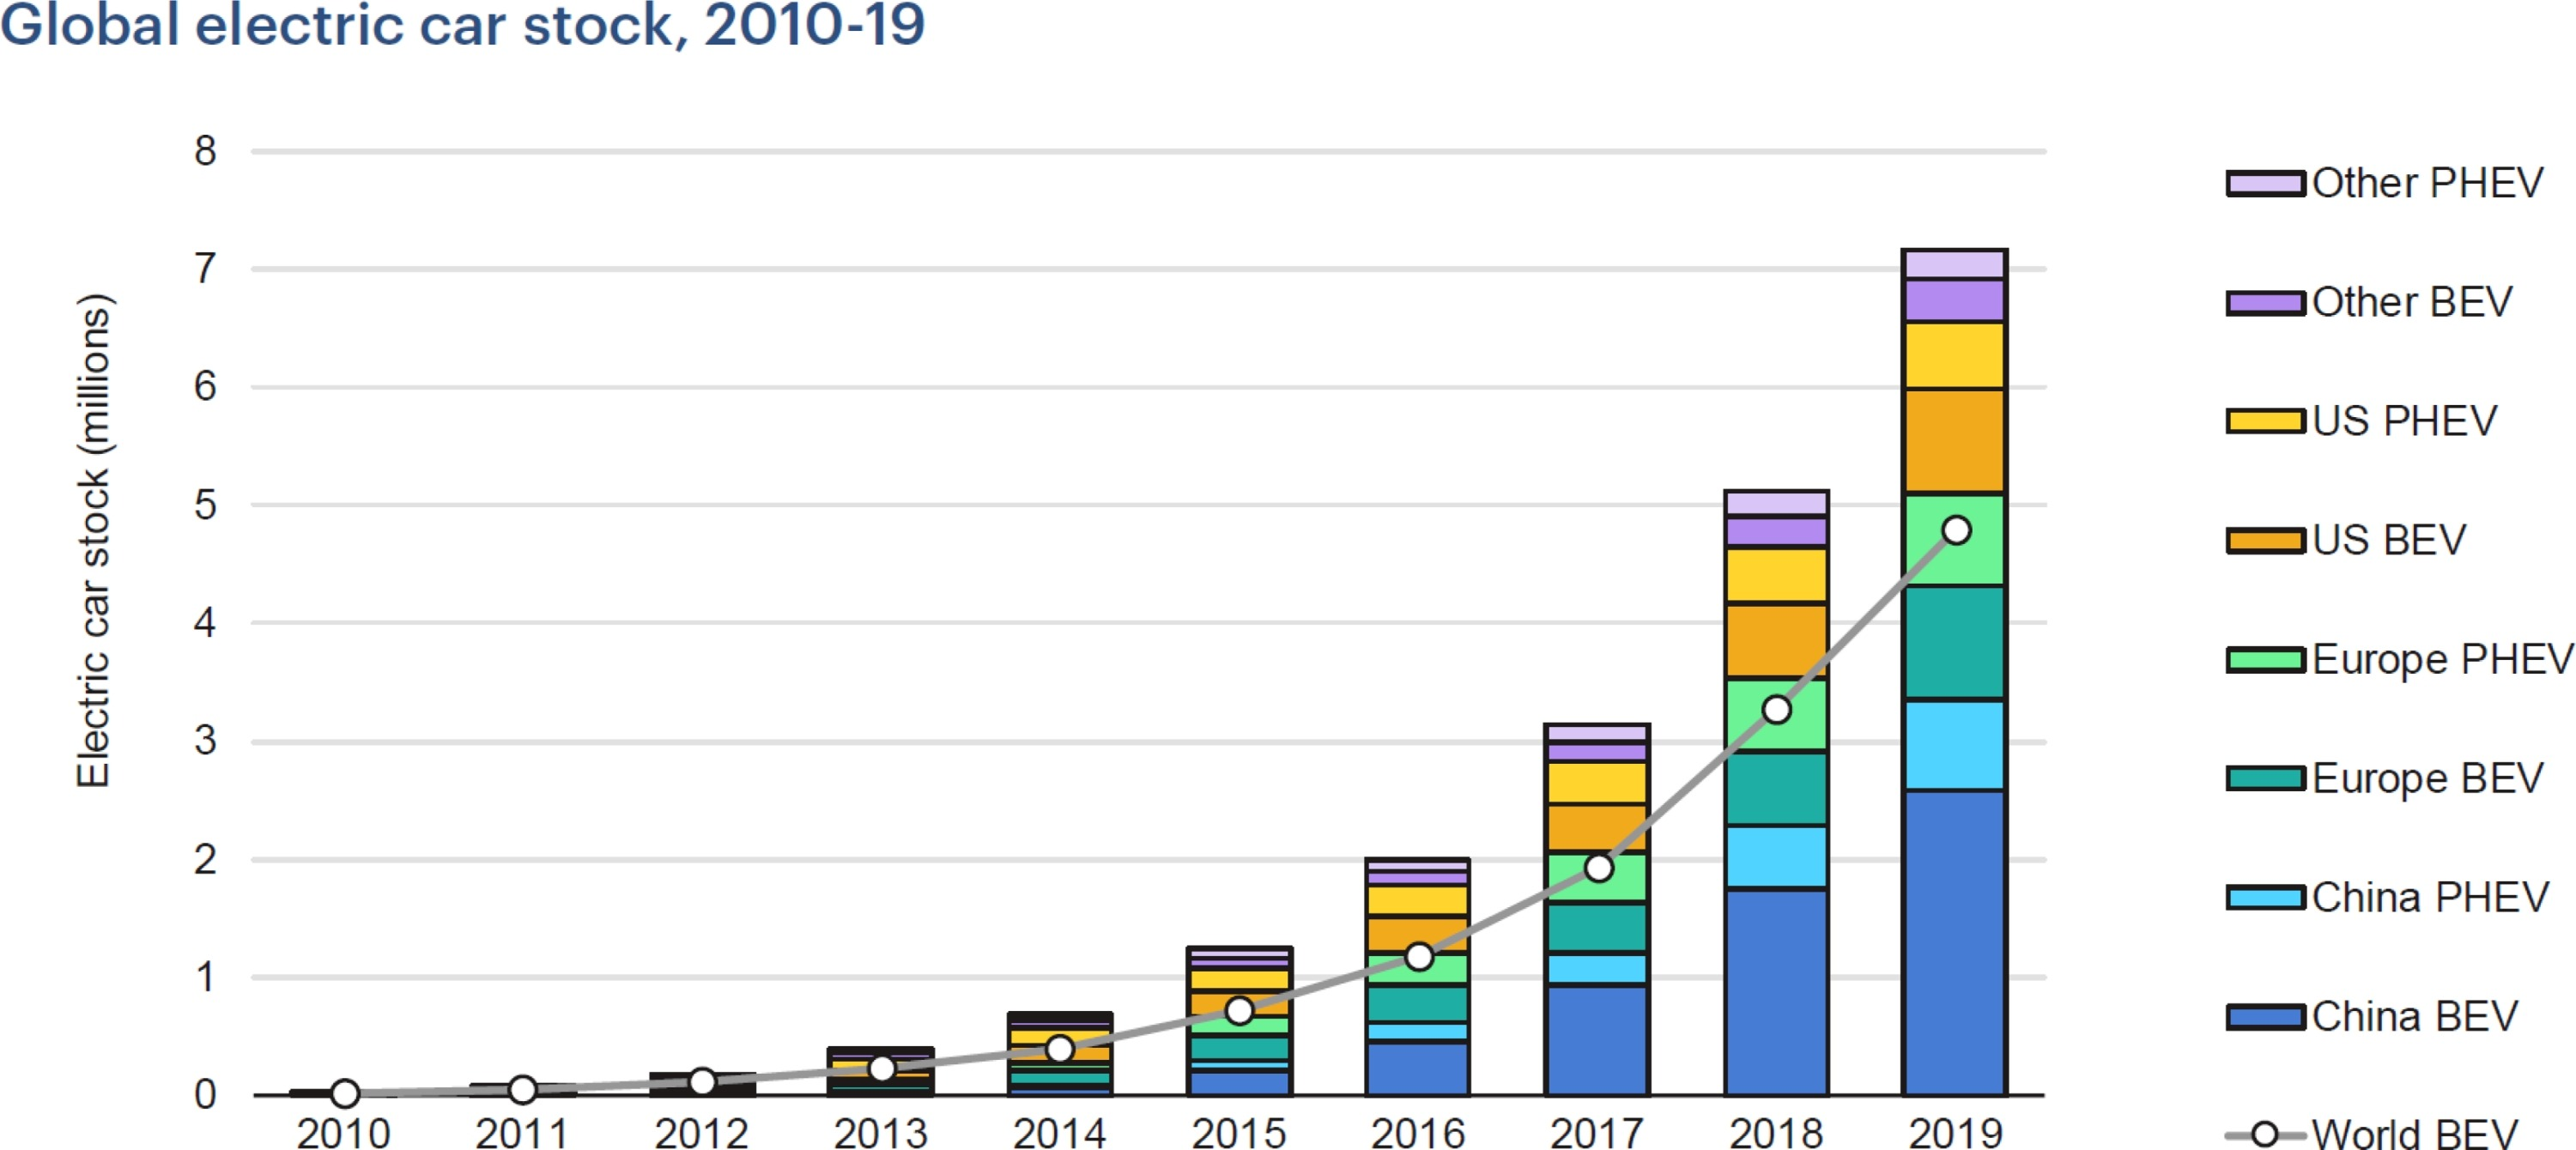
\includegraphics[scale=0.7]{figures/Figure/Global_electric car stock.jpg}
    \caption{Global electric car stock}
\end{figure}

From the graph, it is evident that the collected data exhibits characteristics of a linear log-log function. Considering this characteristic, we may contemplate using a linear log-log regression model for fitting.
\begin{figure}[htbp]
    \centering
    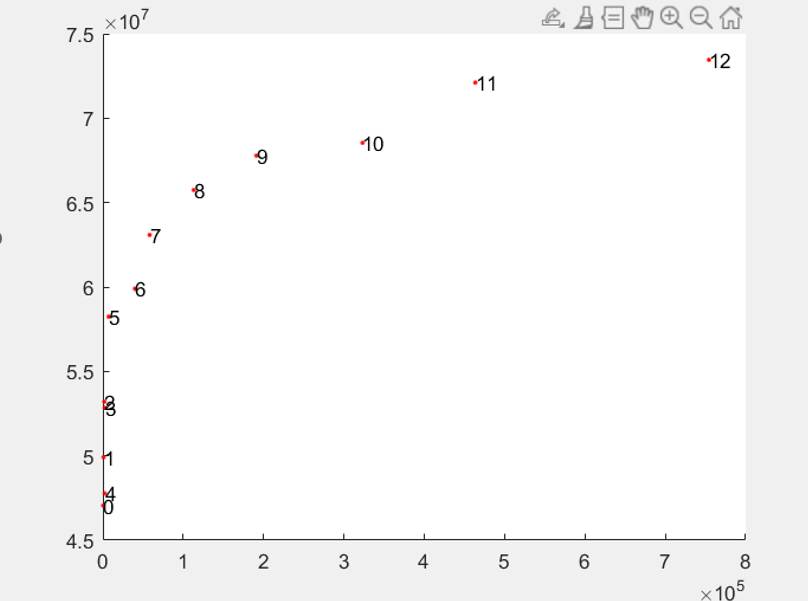
\includegraphics[scale=0.5]{figures/Figure/scatter.png}
    \caption{Scatter}
\end{figure}


\subsubsection{Exponential Fitting Model Introduction}
The general form of the exponential curve prediction model is:
\[ \hat{y} = ae^{bx} \]
Where:
\( \hat{y} \) is the predicted value.

\( x \) is the independent variable.

\( a \) and \( b \) are model parameters.

\( e \) is the natural logarithm.

\noindent The fitting function is given by:
\[ f(x) = (3.436 \times 10^7) \cdot x^{0.05465} \]

The fitted model results are as follows:
\[ \text{SSE} = 5.459 \times 10^{13} \]
\[ \text{R-square} = 0.9515 \]
\[ \text{RMSE} = 2.133 \times 10^6 \]

It can be observed that the R-square is close to 1, but the large values of RMSE and SSE indicate a relatively poor fit. Next, we will attempt to fit the data using a linear double-logarithmic regression model.

\subsubsection{Logarithmic Regression Curve }
The double logarithmic regression curve is expressed as follows:
\[ \ln(y) = a + b \ln(x) \]

Where \( a \) and \( b \) are the model parameters. The data can be first transformed by taking the logarithm, and then a linear regression can be applied. Let
\[ c_i = \ln(x_i) \]
\[ d_i = \ln(y_i) \]

Then, the parameter \( b \) is calculated by the formula:
\[ b = \frac{\sum_{i=1}^n (d_i - \bar{d})(c_i - \bar{c})}{\sum_{i=1}^n (c_i - \bar{c})^2} \]

Here, \( \bar{d} \) and \( \bar{c} \) are the mean values of \( d_i \) and \( c_i \) respectively.

ln(y)=17.32+0.05806ln(x)
The transformed equation is given by:
\[ y = x^{0.05806} \cdot e^{17.32} \]

\begin{figure}[htbp]
    \centering
    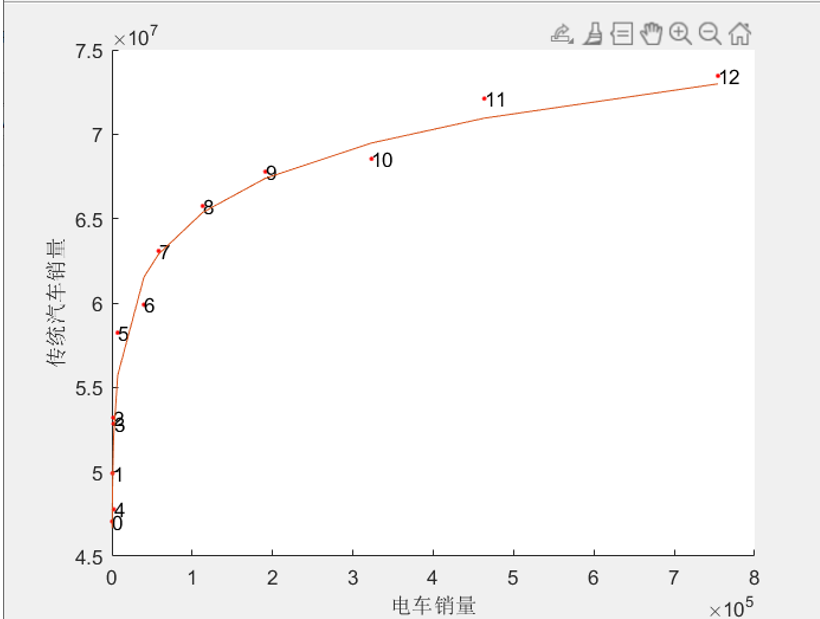
\includegraphics[scale=0.5]{figures/Figure/log.png}
    \caption{Log fiiting}
\end{figure}
This fitted model shows a very good performance as evidenced by the R-square being close to 1, and the small values of RMSE and SSE approaching zero. The curve of the fitted function closely adheres to the distribution of the data points, indicating an excellent fit.

Observing the fitted curve, it conforms well to the pattern of the data points, confirming the effectiveness of the fit. The relationship between the development of traditional cars and new energy electric vehicles is suggested to be a power function. As the development of new energy electric vehicles progresses, the growth of traditional cars is expected to gradually slow down and eventually stabilize.

\subsection{Question4}

\subsubsection{Policy collection}
France plans to reallocate electric vehicle subsidies to reward consumers purchasing electric vehicles manufactured in Europe. Starting March 2023, a 40% tariff has been imposed on electric vehicles imported from China. In 2022, the U.S. Congress passed the "Inflation Reduction Act," stating that electric vehicles with battery components manufactured or assembled by "concerned foreign entities" would not qualify for a $7,500 tax credit. Since the signing of the "2022 Inflation Reduction Act" by the U.S. on August 16, 2022, eight multinational car companies have expressed their stance on the U.S. electric vehicle subsidy protection policy.

Many countries, to protect their domestic industries, have implemented restrictive measures against China's new energy electric vehicles. These measures are expected to limit the growth of China's new energy electric vehicle exports.

We collected information on China's new energy vehicle exports from the General Administration of Customs of China. This data is used to explore the impact of foreign resistance policies on China's new energy vehicle exports.

\subsubsection{Grey Forecasting}
The process of grey forecasting is illustrated in the Figure18.

\begin{figure}[htbp]
    \centering
    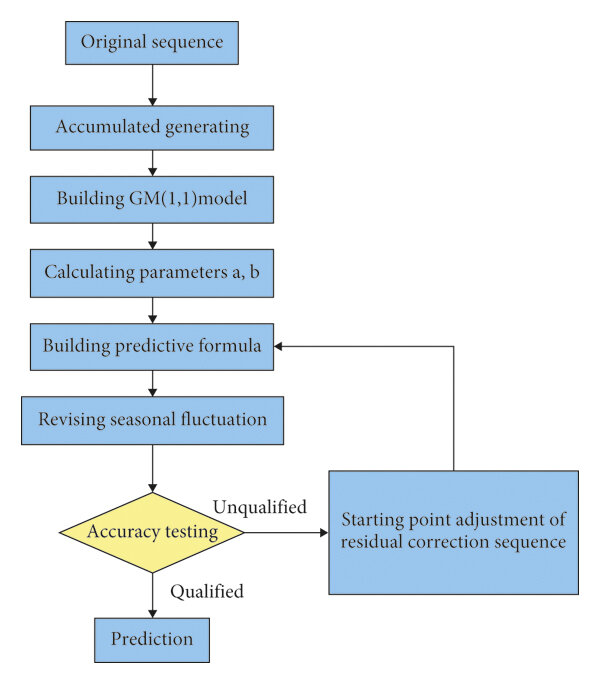
\includegraphics[scale=1]{figures/Figure/Grayl.png}
    \caption{Gray Prediction Framework}
\end{figure}


The fitting result is illustrated in the Figure 19.

\begin{figure}[htbp]
    \centering
    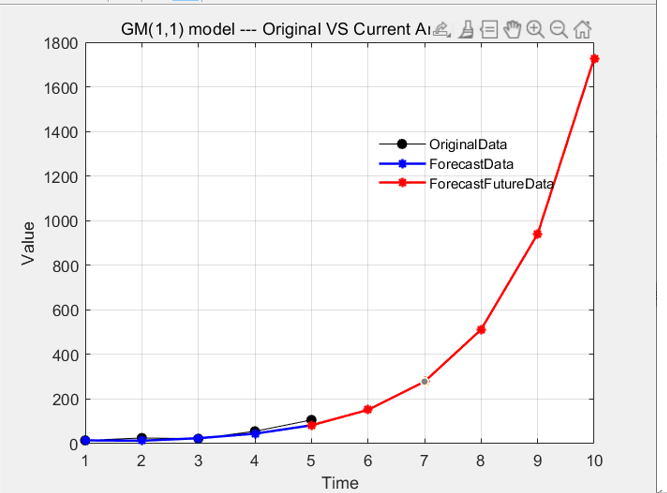
\includegraphics[scale=1]{figures/Figure/result.png}
    \caption{Gray Prediction result}
\end{figure}

The fitted values are: a small probability error P=1, a coefficient of variation C=0.2788, and the prediction grade is: good. The correlation degree R=0.6424 is within an acceptable range. Overall, the forecasting performance is quite good. Through fitting the data, it is evident that even in the face of foreign policy restrictions, the export volume of China's new energy vehicles is expected to increase year by year, with an estimated breakthrough of 2.7 million in 2024.

\subsection{Question5 and Question6}
We visualize the impact of the production and sales of new energy vehicles on the environment, with our quantifiable indicators for the environment being carbon dioxide emissions and air quality index.
Figure 20.a represents the reduction in carbon dioxide emissions, while Figure 20.b represents carbon dioxide emissions. The relationship between the air quality index in Beijing, and the production and sales of new energy vehicles changes over time.

\begin{figure}[htbp]
    \centering
    \subfigure[]{
    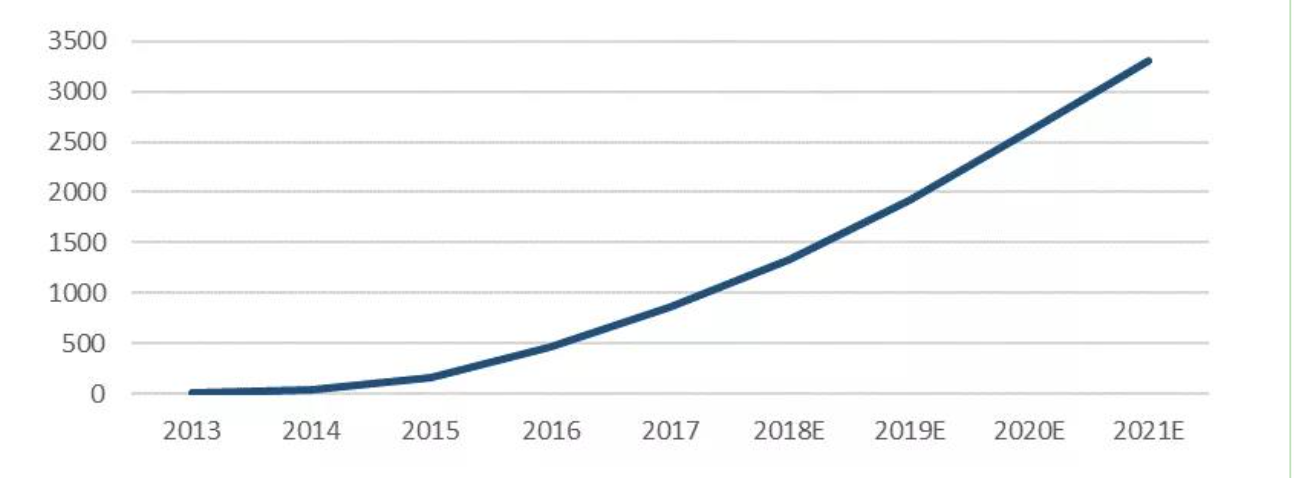
\includegraphics[scale=0.3]{figures/Figure/减排量1.png} \label{1}
    }
    \quad
    \subfigure[]{
    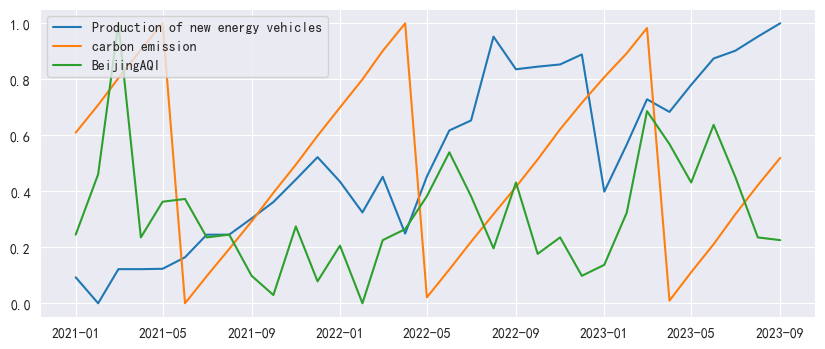
\includegraphics[scale=0.3]{figures/Figure/pcb.png} \label{2} 
    }
    \caption{}
    \end{figure}

We utilize the Life Cycle Assessment (LCA) method with CO2 emissions as the ecological environmental assessment indicator to evaluate the impact of electric vehicles on the environment. The LCA process includes five stages: raw material acquisition, production, transportation, use and maintenance, and end-of-life recycling.
The Life Cycle Assessment framework typically involves four stages: determination of goals and scope boundaries (establishing the functional unit), inventory analysis (data collection and modeling), impact assessment (calculation), and interpretation of results.\cite{HZ}

\begin{figure}[htbp]
    \centering
    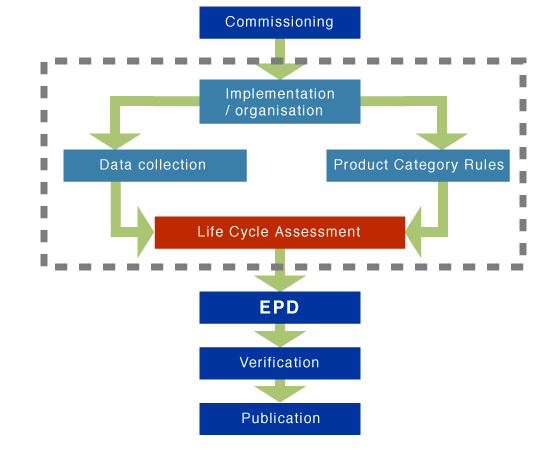
\includegraphics[scale=0.5]{figures/Figure/LCA2.png}
    \caption{LCA Framework}
\end{figure}
The life cycle assessment framework typically involves four stages: determining goals and scope boundaries (establishing the functional unit), conducting inventory analysis (data collection and modeling), performing impact assessment (calculation), and interpreting results.\cite{1234}

We have selected pure electric diesel-electric buses as the assessment subject. Based on the LCA framework, we use carbon emission coefficients as indicators, measured in grams of carbon dioxide equivalent per kilogram of substance (CO2eq/kg). The formulas for each stage of the bus's life cycle are as follows.


The translation of the formula for calculating the carbon emissions in the fuel production and transportation lifecycle \cite{1234} is:
$I_f = C_e * E * S$

$I_f$ represents the carbon emissions during the fuel production and transportation process; "Ce" represents the carbon equivalent emission coefficient for the fuel; "E" represents energy utilization efficiency; "S" represents the proportion of energy consumption structure. \\

The translation of the formula for calculating carbon emissions during the operation phase of buses \cite{unep2019emissions} is:
$I_u = \frac{FE*EF*U}{TE}$

$I_u$ represents the carbon emissions during the operational phase of the bus; FE represents the fuel or electricity consumption per hundred kilometers of the bus; EF represents the carbon emissions per unit of electricity or diesel; U is the distance traveled by the bus; TE represents the charging efficiency or fuel transmission efficiency.


The translation of the formula for calculating carbon emissions during the recycling process of buses \cite{47} is:
$I_{re} = \sum_{i=1}^{n}(-M_i*\beta * (i_{pi}-i_{si}))$

$I_{re}$ represents the carbon emissions during the recycling process of the bus; $I_{pi}$ represents the unit carbon emissions recycled during the vehicle material production process; $I_{si}$ represents the unit carbon emissions recycled after the disposal of vehicle materials; $M_i$ represents the mass of different materials; $\beta$ represents the recycling-related carbon emission coefficient.
For simplicity in calculations, we assume that the recycled material is only flat carbon steel.
The model parameters are as shown in Table 2.
\begin{longtable}{c|c|c}
    \hline
    parameters      &  Electric Bus  & Oil Bus  \\ \hline
    $C_e$           &  98600g/kg          &  98600g/kg        \\
    $E$             &    90\%            &  25\%        \\
    $S$             &    15.9\%            &    67\%       \\
    $FE$            &    120kWh /100km  &  40L /100km           \\
    $EF$            &    4.74kg/km            &105.8kg /km          \\
    $U$             &     95 ten thousand km      &  95 ten thousand km         \\
    $TE$            &     90\%           &  100\%          \\
    $M_i$           &      5160          &   5719         \\
    $\beta$         &      1.87          &   0.399         \\ \hline

\end{longtable}
According to the bus situation in Hangzhou, we infer that in a city with a population of one million, there are a total of 250 pure electric buses and 270 diesel buses. The model's calculation results indicate that the carbon emissions of pure electric buses over their lifecycle amount to 275.75 tons, while diesel buses emit 350.25 tons of carbon over their lifecycle. We observe that pure electric buses achieve a carbon emission reduction rate of 21.428\%.

From this, it can be seen that the widespread adoption of new energy electric buses in cities has a significant improvement on the ecological environment, especially in terms of carbon emissions and air quality indices.

\subsubsection{Towards a Clean Future: The Ecological Choice of New Energy Electric Vehicles}

\noindent Dear citizens,

I am writing this letter to share with you some good news about new energy electric vehicles and the significant contributions this industry has made globally. Recent research indicates that new energy electric vehicles have had a positive impact on improving our ecological environment.

According to our analysis, new energy electric vehicles play a crucial role in improving air quality and reducing greenhouse gas emissions. By replacing traditional fuel vehicles, new energy electric vehicles can significantly decrease CO2 emissions annually, creating a cleaner and healthier living environment for our cities. This means fresher air and greener cities, beneficial for the health and well-being of us all.

We encourage every citizen to consider incorporating new energy electric vehicles into their lifestyles. By choosing new energy electric vehicles, we not only make a positive contribution to the environment on an individual level but also support this thriving industry, contributing to the sustainable future of our cities.

Let's work together for a clean, green future. Thank you for your support and cooperation.

Warm regards,

\section{Conclusions}

\subsection{Conclusions of the problem}
After a thorough analysis, we have found that the development of new energy vehicles is influenced by various factors, including policies, economics, environment, infrastructure, and energy. By establishing a model, we predict that China's new energy vehicles will experience rapid development in the next decade, with the growth rate of production and sales continually accelerating.

In further studies, we discovered that the rise of new energy vehicles has imposed constraints on the global traditional energy vehicle industry, evident in production and sales volumes as well as patent numbers. Additionally, our analysis of foreign resistance policies against China's new energy vehicles revealed that while these policies have slowed down the development of our country's new energy vehicles to some extent, overall, the industry continues to demonstrate robust momentum and is unstoppable.

Finally, by employing the life cycle assessment method, we have determined the emission reduction amount and rate achieved by electric buses throughout their entire life cycle. The results indicate that new energy electric vehicles can efficiently improve the ecological environment, creating a more beautiful living environment for the general public.

\subsection{Methods used in our models}
In our exploration of the factors influencing new energy vehicles, we adorned our analytical toolkit with the sophisticated Grey Relational Analysis (GRA) model and the robust Multiple Linear Regression model. Delving into the intricate relationships within time series, we harnessed the power of the Long Short-Term Memory (LSTM) and AutoRegressive Integrated Moving Average (ARIMA) models. For the nuanced task of predicting small-sample data, we gracefully employed the Grey Prediction model. Finally, to quantitatively assess the ecological impact of new energy vehicles, we seamlessly integrated the comprehensive Life Cycle Assessment (LCA) method.




\bibliographystyle{unsrt}
\bibliography{ref.bib}



%参考文献
\newpage
%附录

\section{Appendix}
\begin{lstlisting}[language=matlab,caption={The matlab Source code of Algorithm}]
    function gm11 = GM11_model(X,td)
    n  = length(X);    
    Ago = cumsum(X);   
    Z = (Ago(1:end-1) + Ago(2:end) ) / 2; 
    Yn = X(2:end)';
    B= [-Z;ones(1,n-1)]'; 
    LS_solution = (B'*B)\(B'*Yn); 
    a = LS_solution(1);   
    u = LS_solution(2); 
    F = [X(1),(X(1)-u/a)./exp(a*(1:n+td-1))+u/a];
    PreData = [F(1),F(2:end)-F(1:end-1)];
    t = 1:n;
    plot(t,X,'ko-','MarkerFaceColor','k')  
    hold on;
    grid on
    plot(t,PreData(1:n),'b*-','LineWidth',1.5)  
    plot(n:n+td,PreData(n:n+td),'r*-','LineWidth',1.5)
    title('GM(1,1) model --- Original VS Current And Future Predict');
    legend('OriginalData','ForecastData','ForecastFutureData','Location','best')
    legend('boxoff')
    set(get(gca, 'XLabel'), 'String', 'Time');
    set(get(gca, 'YLabel'), 'String', 'Value');
    Err = abs(X-PreData(1:n));  
    q = mean(Err./X);
    XVar = std(X,1);
    ErrVar = std(Err(2:end):1);
    C = ErrVar/XVar; 
    P = sum(abs(Err-mean(Err))<0.6745*XVar)/n;  
    R_k = (min(Err)+0.5*max(Err))./(Err+0.5*max(Err));
    R = sum(R_k)/length(R_k); 
    gm11.Coeff_a = a;
    gm11.Coeff_u = u;
    gm11.Predict_Value = PreData;
    gm11.AbsoluteError = Err;
    gm11.RelativeErrorMean = q;
    gm11.R = R;
    gm11.C = C;
    gm11.P = P;
   end
   
\end{lstlisting}
\begin{lstlisting}[language=Python,caption={The Python Source code of Algorithm}]
    import numpy as np
    import pandas as pd
    pd.set_option('display.float_format', lambda x: '{:.2f}'.format(x))
    import seaborn as sns
    color = sns.color_palette()
    sns.set_style('darkgrid')
    import matplotlib.pyplot as plt
    plt.rcParams["font.sans-serif"]=["SimHei"] #设 置 字 体
    plt.rcParams["axes.unicode_minus"]=False #该 语 句 解 决 图 像中 的 “ -” 负 号 的 乱 码 问 题
    %matplotlib inline
    from scipy import stats
    from scipy.special import boxcox1p
    from scipy.stats import norm, skew
    import warnings
    def ignore_warn(*args, **kwargs):
        pass
    warnings.warn = ignore_warn
    import scipy.stats as stats
    from scipy.stats import shapiro, skew
    import math
    import plotly.express as px
    import plotly.graph_objs as go
    import plotly.subplots as sp
    from plotly.subplots import make_subplots
    import plotly.figure_factory as ff
    from IPython.display import display
    from plotly.offline import init_notebook_mode
    init_notebook_mode(connected=True)
    seed = 42
    plotly_template = 'simple_white'
    df = pd.read_excel("../Data/新能源汽车产销量.xlsx")
    f, ax = plt.subplots(nrows=1, ncols=1, figsize=(16,5))
    
    sns.heatmap(df.T.isna(), cmap='Blues')
    ax.set_title('Missing Values', fontsize=16)
    
    for tick in ax.yaxis.get_major_ticks():
        tick.label.set_fontsize(14)
    plt.show()
    # 对整个 DataFrame 进行中位数填充
    df = df.fillna(df.median())
    def describe(df):
        '''
        This function plots a table containing Descriptive Statistics of the Dataframe
        '''
        mean_features = df.mean().round(2).apply(lambda x: "{:,.2f}".format(x)) 
        std_features = df.std().round(2).apply(lambda x: "{:,.2f}".format(x)) 
        q1 = df.quantile(0.25).round(2).apply(lambda x: "{:,.2f}".format(x))
        median = df.quantile(0.5).round(2).apply(lambda x: "{:,.2f}".format(x))
        q3 = df.quantile(0.75).round(2).apply(lambda x: "{:,.2f}".format(x))
    
    
        # Generating new Dataframe
        describe_df = pd.DataFrame({'Feature Name': mean_features.index,
                                    'Mean': mean_features.values,
                                    'Standard Deviation': std_features.values,
                                    '25%': q1.values,
                                    'Median': median.values,
                                    '75%': q3.values})
    
        # Generating a Table w/ Pyplot
        fig = go.Figure(data = [go.Table(header=dict(values=list(describe_df.columns),
                                                     align = 'center',
                                                     fill_color = 'midnightblue',
                                                   font=dict(color = 'white', size = 18)),
                                         cells=dict(values=[describe_df['Feature Name'],
                                                            describe_df['Mean'],
                                                            describe_df['Standard Deviation'],
                                                           describe_df['25%'],
                                                           describe_df['Median'],
                                                           describe_df['75%']],
                                                    fill_color = 'gainsboro',
                                                    align = 'center'))
                               ])
    
        fig.update_layout(title = {'text': f'<b>Descriptive Statistics of the Dataframe<br><sup> (Mean, Standard Deviation, 25%, Median, and 75%)</sup></b>'},
                          template = plotly_template,
                          height = 700, width = 950,
                          margin = dict(t = 100))
    
        fig.show()
    
    def plot_boxplot_matrix(df):
        
        '''
        This function identifies all continuous features within the dataset and plots
        a matrix of boxplots for each attribute
        '''
        
        continuous_features = []
        for feat in df.columns:
            if df[feat].nunique() > 2:
                continuous_features.append(feat)
        
        num_cols = 2
        num_rows = (len(continuous_features) + 1) // num_cols
    
    
        fig = make_subplots(rows=num_rows, cols=num_cols)
    
    
        for i, feature in enumerate(continuous_features):
            row = i // num_cols + 1
            col = i % num_cols + 1
    
            fig.add_trace(
                go.Box(
                    x=df[feature],
                    name = ' '
                ),
                row=row,
                col=col
            )
    
            fig.update_yaxes(title_text = ' ', row=row, col=col)
            fig.update_xaxes(title_text= feature, row=row, col=col)
            fig.update_layout(
                title=f'<b>Boxplot Matrix<br> <sup> Continuous Features</sup></b>',
                showlegend=False,
                yaxis=dict(
                tickangle=-90  
            )
            )
    
        fig.update_layout(
            height=350 * num_rows,
            width=1000,
            margin=dict(t=100, l=80),
            template= plotly_template
        )
    
    
        fig.show()
    plot_boxplot_matrix(df)
    柱状图
    def plot_histogram_matrix(df):
        
        '''
        This function identifies all continuous features within the dataset and plots
        a matrix of histograms for each attribute
        '''
        
        continuous_features = []
        for feat in df.columns:
            if df[feat].nunique() > 2:
                continuous_features.append(feat)
        num_cols = 2
        num_rows = (len(continuous_features) + 1) // num_cols
    
        fig = make_subplots(rows=num_rows, cols=num_cols)
    
        for i, feature in enumerate(continuous_features):
            row = i // num_cols + 1
            col = i % num_cols + 1
    
            fig.add_trace(
                go.Histogram(
                    x=df[feature],
                    name=feature
                ),
                row=row,
                col=col
            )
    
            fig.update_xaxes(title_text=feature, row=row, col=col)
            fig.update_yaxes(title_text='Frequency', row=row, col=col)
            fig.update_layout(
                title=f'<b>Histogram Matrix<br> <sup> Continuous Features</sup></b>',
                showlegend=False
            )
    
        fig.update_layout(
            height=350 * num_rows,
            width=1000,
            margin=dict(t=100, l=80),
            template= plotly_template
        )
    
        fig.show()
    plot_histogram_matrix(df)
    def shapiro_wilk_test(df):
        '''
        This function performs a Shapiro-Wilk test to check if the data is normally distributed or not, as well as skewness
        '''
        print(f'\033[1mShapiro-Wilk Test & Skewness:\033[0m')
        print('\n- - - - - - - - - - - - - - - - - - - - - - - - - - - - - - - - - - - - - - - - - - - - - - - - - - - -  \n')
    
        numeric_columns = df.select_dtypes(include=['float', 'int']).columns
    
        for feature in numeric_columns:
            stats, p_value = shapiro(df[feature])
    
            if p_value < 0.05:
                text = f'{feature} Does Not Seem to be Normally Distributed'
            else:
                text = f'{feature} Seems to be Normally Distributed'
    
            print(f'{feature}')
            print(f'\n  Shapiro-Wilk Statistic: {stats:.2f}')
            print(f'\n  Shapiro-Wilk P-value: {p_value}')
            print(f'\n  Skewness: {np.round(skew(df[feature]), 2)}')
            print(f'\n  Conclusion: {text}')
            print('\n===============================================================================================')
    
        print('\n- - - - - - - - - - - - - - - - - - - - - - - - - - - - - - - - - - - - - - - - - - - - - - - - - - - -  \n')
        print(f'\033[1mEnd of Shapiro-Wilk Test\033[0m')
    shapiro_wilk_test(df)
    相关性热力图
    import plotly.figure_factory as ff
    import plotly.express as px
    import plotly.graph_objs as go
    import plotly.subplots as sp
    from plotly.subplots import make_subplots
    import plotly.figure_factory as ff
    from IPython.display import display
    from plotly.offline import init_notebook_mode
    init_notebook_mode(connected=True)
    def plot_correlation(df):
        '''
        This function is resposible to plot a correlation map among features in the dataset
        '''
        corr = np.round(df.corr(), 2)
        mask = np.triu(np.ones_like(corr, dtype = bool))
        c_mask = np.where(~mask, corr, 100)
    
        c = []
        for i in c_mask.tolist()[1:]:
            c.append([x for x in i if x != 100])
        
        fig = ff.create_annotated_heatmap(z=c[::-1],
                                          x=corr.index.tolist()[:-1],
                                          y=corr.columns.tolist()[1:][::-1],
                                          colorscale = 'bluyl')
    
        fig.update_layout(title = {'text': '<b>Feature Correlation <br> <sup>Heatmap</sup></b>'},
                          height = 1050, width = 1050,
                          margin = dict(t=210, l = 80),
                          template = 'simple_white',
                          yaxis = dict(autorange = 'reversed'))
    
        fig.add_trace(go.Heatmap(z = c[::-1],
                                 colorscale = 'bluyl',
                                 showscale = True,
                                 visible = False))
        
        
        
        fig.data[1].visible = True
    
        fig.show()
    plot_correlation(df)
    from datetime import date
    
    
    f, ax = plt.subplots(nrows=18, ncols=1, figsize=(15, 80))
    
    for i, column in enumerate(df.drop('date', axis=1).columns):
        sns.lineplot(x=df['date'], y=df[column].fillna(method='ffill'), ax=ax[i], color='dodgerblue')
        ax[i].set_title('Feature: {}'.format(column), fontsize=14)
        ax[i].set_ylabel(ylabel=column, fontsize=14)
        ax[i].set_xlim([date(2020, 11, 1), date(2023, 8, 1)])  
    import statsmodels.api as sm
    
    # 假设 X 是包含三个自变量的特征矩阵,Y 是因变量
    X = df[['Output of power batteries', 'Number of public charging piles_DC piles', 'Subsidy policy','International energy market prices', 'BeijingAQI']]
    y = df['Production of new energy vehicles']
    model = sm.OLS(y, X).fit()  # 拟合最小二乘回归模型
    
    # 打印回归系数的摘要
    print(model.summary())
    
    y_pred = model.predict(X)
    
    # 绘制原始数据和拟合曲线
    plt.scatter(df['date'], y, label='Actual data')
    plt.plot(df['date'], y_pred, color='red', label='Fit line')
    
    plt.xlabel('date')
    plt.ylabel('Production of new energy vehicles')
    plt.title('Multiple Linear Regression Fit')
    plt.legend()
    plt.show()
    from sklearn.preprocessing import MinMaxScaler
    
    # 创建 MinMaxScaler 对象
    scaler = MinMaxScaler()
    
    # 假设 df 是包含要归一化的数据的 DataFrame
    # 列名为 'Output of power batteries', 'Number of public charging piles_DC piles', 'Subsidy policy', 'International energy market prices', 'BeijingAQI'
    columns_to_normalize = ['Production of new energy vehicles','carbon emission','BeijingAQI']
    
    # 使用 Min-Max 归一化对指定列进行处理
    df[columns_to_normalize] = scaler.fit_transform(df[columns_to_normalize])
    
    plt.figure(figsize=(10,4))
    plt.plot(df.date, df['Production of new energy vehicles'], label="Production of new energy vehicles")
    plt.plot(df.date, df['carbon emission'], label="carbon emission")
    plt.plot(df.date, df['BeijingAQI'], label="BeijingAQI")
    plt.legend()

    import numpy as np
    import pandas as pd
    pd.set_option('display.float_format', lambda x: '{:.2f}'.format(x))
    import seaborn as sns
    color = sns.color_palette()
    sns.set_style('darkgrid')
    import matplotlib.pyplot as plt
    plt.rcParams["font.sans-serif"]=["SimHei"] #设 置 字 体
    plt.rcParams["axes.unicode_minus"]=False #该 语 句 解 决 图 像中 的 “ -” 负 号 的 乱 码 问 题
    %matplotlib inline
    from scipy import stats
    from scipy.special import boxcox1p
    from scipy.stats import norm, skew
    import warnings
    def ignore_warn(*args, **kwargs):
        pass
    warnings.warn = ignore_warn
    import scipy.stats as stats
    from scipy.stats import shapiro, skew
    import math
    
    # Re-loads all imports every time the cell is ran. 
    %load_ext autoreload
    %autoreload 2
    
    from time import time
    
    import numpy as np
    import pandas as pd
    pd.options.display.float_format = '{:,.5f}'.format
    
    from IPython.display import display
    
    # Sklearn tools
    from sklearn.model_selection import train_test_split
    from sklearn.preprocessing import StandardScaler
    
    # Neural Networks
    import torch
    import torch.nn as nn
    
    from torch.utils.data import Dataset, DataLoader
    
    import pytorch_lightning as pl
    from pytorch_lightning import Trainer, seed_everything
    from pytorch_lightning.loggers.csv_logs import CSVLogger
    
    # Plotting
    %matplotlib inline
    import matplotlib.pyplot as plt
    df = pd.read_excel("../Data/新能源汽车产销量.xlsx")
    df_date = df[['date', 'Production of new energy vehicles']]
    df_date.set_index(df.date, inplace=True)
    df_date.drop(columns='date', inplace=True)
    test_percent = 0.1
    test_point = np.round(len(df_date)*test_percent)
    test_index = int(len(df_date) - test_point)
    train = df_date.iloc[:test_index]
    test = df_date.iloc[test_index:]
    from sklearn.preprocessing import MinMaxScaler
    scaler = MinMaxScaler()
    scaler.fit(train)
    scaled_train = scaler.transform(train)
    scaled_test = scaler.transform(test)
    from tensorflow.keras.preprocessing.sequence import TimeseriesGenerator
    from tensorflow.keras.models import Sequential
    from tensorflow.keras.layers import Dense, LSTM
    from tensorflow.keras.callbacks import EarlyStopping
    early_stop = EarlyStopping(monitor='val_loss',patience=2)
    length = 6
    generator = TimeseriesGenerator(scaled_train,scaled_train,
                                   length=length,batch_size=1)
    
    
    validation_generator = TimeseriesGenerator(scaled_test,scaled_test,
                                              length=length,batch_size=1)
    n_features = 1
    model = Sequential()
    model.add(LSTM(12, input_shape = (length, n_features)))
    model.add(Dense(1))
    model.compile(optimizer = 'adam', loss = 'mse')
    model.fit_generator(generator, epochs = 10, 
                        validation_data = validation_generator, 
                        callbacks = [early_stop])
    model.save('model_LSTM.h5')
    loss = pd.DataFrame(model.history.history)
    loss.plot()
    prediction = []
    evaluation_batch = scaled_train[-length:]
    current_batch = evaluation_batch.reshape(1, length, n_features)
    for i in range (len(test)):
        current_prediction = model.predict(current_batch)[0]
        prediction.append(current_prediction)
        current_batch = np.append(current_batch[:, 1:, :], [[current_prediction]], axis = 1)
    prediction = scaler.inverse_transform(prediction)
    test['LSTM Prediction'] = prediction
    test.plot(figsize = (10, 4))
    full_scaler = MinMaxScaler()
    full_data_scale = scaler.transform(df_date)
    length = 50 
    generator = TimeseriesGenerator(full_data_scale, full_data_scale, length=length, batch_size=1)
    model = Sequential()
    model.add(LSTM(50, input_shape=(length, n_features)))
    model.add(Dense(1))
    model.compile(optimizer='adam', loss='mse')
    model.fit_generator(generator,epochs=6)
    prediction = []
    evaluation_batch = full_data_scale[-length:]
    current_batch = evaluation_batch.reshape(1, length, n_features)
    for i in range (120):
        current_prediction = model.predict(current_batch)[0]
        prediction.append(current_prediction)
        current_batch = np.append(current_batch[:, 1:, :], [[current_prediction]], axis = 1)
    prediction = scaler.inverse_transform(prediction)
    
    len(prediction)
    from datetime import timedelta
    from datetime import datetime
    date_string = "2023-09"
    date_format = "%Y-%m"
    datetime_object = datetime.strptime(date_string, date_format)
    future_months = [datetime_object + timedelta(days=30 * i) for i in range(1, 121)]
    future_months
    prediction_index = future_months
    plt.plot(df_date.index,df_date['Production of new energy vehicles'])
    plt.plot(prediction_index,prediction)
    prelist = []
    for i in prediction:
        prelist.append(i[0])
    start_date = datetime(2023, 10, 1)
    
    # 生成未来十年的日期列表(每个月)
    date_list = [start_date + timedelta(days=30 * i) for i in range(10 * 12)]
    date_list
    forecast = pd.DataFrame(data={'forecast':prelist, 'Date': date_list})
    forecast.to_csv("../result/prediction_lstm.csv")
    import pandas as pd
    import numpy as np
    import matplotlib.pyplot as plt
    %matplotlib inline
    import seaborn as sns
    from datetime import datetime
    pd.options.display.float_format = '{:.2f}'.format
    from tqdm import tqdm
    import warnings
    warnings.filterwarnings('ignore')
    import pickle
    
    from itertools import combinations
    from statsmodels.tsa.stattools import adfuller
    from statsmodels.tsa.stattools import acf, pacf
    from statsmodels.tsa.arima.model import ARIMA as ARIMA
    import statsmodels.api as sm
    import statsmodels.tsa.api as smt
    def test_stationarity(timeseries):
        #Determing rolling statistics
        MA = timeseries.rolling(window=12).mean()
        MSTD = timeseries.rolling(window=12).std()
    
        #Plot rolling statistics:
        plt.figure(figsize=(15,5))
        orig = plt.plot(timeseries, color='blue',label='Original')
        mean = plt.plot(MA, color='red', label='Rolling Mean')
        std = plt.plot(MSTD, color='black', label = 'Rolling Std')
        plt.legend(loc='best')
        plt.title('Rolling Mean & Standard Deviation')
        plt.show(block=False)
    
        #Perform Dickey-Fuller test:
        print('Results of Dickey-Fuller Test:')
        dftest = adfuller(timeseries, autolag='AIC')
        dfoutput = pd.Series(dftest[0:4], index=['Test Statistic','p-value','#Lags Used','Number of Observations Used'])
        for key,value in dftest[4].items():
            dfoutput['Critical Value (%s)'%key] = value
        print(dfoutput)
    def tsplot(y, lags=None, figsize=(12, 7), style='bmh'):
        if not isinstance(y, pd.Series):
            y = pd.Series(y)
            
        with plt.style.context(style):    
            fig = plt.figure(figsize=figsize)
            layout = (2, 2)
            ts_ax = plt.subplot2grid(layout, (0, 0), colspan=2)
            acf_ax = plt.subplot2grid(layout, (1, 0))
            pacf_ax = plt.subplot2grid(layout, (1, 1))
            
            y.plot(ax=ts_ax)
            p_value = sm.tsa.stattools.adfuller(y)[1]
            ts_ax.set_title('Time Series Analysis Plots\n Dickey-Fuller: p={0:.5f}'.format(p_value))
            smt.graphics.plot_acf(y, lags=lags, ax=acf_ax)
            smt.graphics.plot_pacf(y, lags=lags, ax=pacf_ax)
            plt.tight_layout()
    dec = sm.tsa.seasonal_decompose(df_date['Production of new energy vehicles'],period = 12,model = 'additive').plot()
    plt.show()
    
    test_stationarity(df_date['Production of new energy vehicles'])
    #### Step 3  差分转平稳
    def stationarity(timeseries): #平稳性处理(timeseries 时间序列)
        ## 差分法,保存成新的列
        diff1 = timeseries.diff(1).dropna()  # 1阶差分 dropna() 删除缺失值
        diff2 = diff1.diff(1).dropna() #在一阶差分基础上再做一次一阶差分,即二阶查分
        ## 画图
        diff1.plot(color = 'red',title='diff 1',figsize=(10,4))
        diff2.plot(color = 'black',title='diff 2',figsize=(10,4))
    
        
        ## 平滑法
        rollmean = timeseries.rolling(window=4,center = False).mean() ## 滚动平均
        rollstd = timeseries.rolling(window=4,center = False).std() ## 滚动标准差
        ## 画图 
        rollmean.plot(color = 'yellow',title='Rolling Mean',figsize=(10,4))
        rollstd.plot(color = 'blue',title='Rolling Std',figsize=(10,4))
        
        return diff1,diff2,rollmean,rollstd
    diff1,diff2,rollmean,rollstd = stationarity(df_date)
    tsplot(diff2['Production of new energy vehicles'])
    from statsmodels.graphics.tsaplots import plot_acf,plot_pacf
    from statsmodels.tsa.stattools import adfuller as ADF
    from statsmodels.stats.diagnostic import acorr_ljungbox
    
    import statsmodels.api as sm
    
    
    def testwhitenoise(data):
        m = 10# 检验10个自相关系数
        acf,q,p = sm.tsa.acf(data,nlags=m,qstat=True)
        out = np.c_[range(1,m+1),acf[1:],q,p]
        output = pd.DataFrame(out,columns=['lag','自相关系数','统计量Q值','p_values'])
        output = output.set_index('lag')# 设置第一列索引名称,可省略重复索引列1
        print(output)
    
    def teststeady(data,count=0):
        res_ADF = ADF(data)
        print('ADF检验结果为:', res_ADF)
        Pv = res_ADF[1]
        if Pv > 0.05:
            print('\033[1;31mP值:%s,原始序列不平稳,要进行差分!\033[0m' % round(Pv,5))
            count = count + 1
            print('\033[1;32m进行了%s阶差分后的结果如下\033[0m' % count)
            data = data.diff(1).dropna()
            teststeady(data,count)
        else:
            print('\033[1;34mP值:%s,原始序列平稳,继续建模\033[0m'% round(Pv,5))
        return data
    testwhitenoise(diff2)
    teststeady(diff2)
    
    def confirm_p_q(data):
        fig = plt.figure(figsize=(8,6))
        testwhitenoise(data)
        train = teststeady(data)
        ax1 = fig.add_subplot(211)
        fig = sm.graphics.tsa.plot_pacf(train, lags=10, ax=ax1)
        ax2 = fig.add_subplot(212)
        fig = sm.graphics.tsa.plot_acf(train, lags=10, ax=ax2)
        plt.show()  ###可视化定阶
    
        pmax = int(len(data) / 10)
        qmax = int(len(data) / 10)
        AIC = sm.tsa.arma_order_select_ic(train,max_ar=pmax,max_ma=qmax,ic='aic')['aic_min_order']
        BIC = sm.tsa.arma_order_select_ic(train,max_ar=pmax,max_ma=qmax,ic='bic')['bic_min_order']
        HQIC = sm.tsa.arma_order_select_ic(train,max_ar=pmax,max_ma=qmax,ic='hqic')['hqic_min_order']
        print('AIC:',AIC)
        print('BIC:',BIC)
        print('HQIC:',HQIC)
        return AIC
    pq = confirm_p_q(diff2)##返回p,q值
    
    from statsmodels.tsa.arima.model import ARIMA as ARIMA
    model = ARIMA(diff2['Production of new energy vehicles'], order = (10,2,7))
    model_fit = model.fit()
    print(model_fit.summary())
    def prediction(data):
        ##tempmodel = ARMA(teststeady(data),pq).fit(disp=-1)
        tempmodel = sm.tsa.arima.ARIMA(data, order=(2,2,7)).fit()
        print(tempmodel.summary())
        #num = 10
        #predictoutside1 = tempmodel.forecast(num)[0]#预测样本外的
        predictoutside2 = tempmodel.predict(len(tempmodel.predict()),len(tempmodel.predict()) + 9,dynamic=True)##也是样本外预测,预测结果一致
        predictinside = tempmodel.predict()##样本内预测
        init_value = diff2.values[0]
    
        fig = plt.figure(figsize=(10, 6))
        predictinside = predictinside.cumsum()##差分还原
        pretrueinside = init_value + predictinside
        startprevalue = list(pretrueinside)[-1]
        predictoutside2 = predictoutside2.cumsum()##差分还原
        pretrueoutside = startprevalue + predictoutside2
        
        ##作图
        plt.plot(diff2.values,label='Original')
        plt.plot([init_value] + list(pretrueinside),label='Prediction')
        X = [i for i in range(len(diff2)-11,len(diff2))]
        #plt.plot(X,[startprevalue] + list(pretrueoutside), label='样本外预测值')
        allpredata = [init_value] + list(pretrueinside) + list(pretrueoutside)
        plt.legend()
        plt.show()
        return tempmodel,allpredata
    preres = prediction(diff2)
    
    from sklearn.metrics import mean_squared_error
    
    # 实际值
    actual_values = diff2.values
    
    # 预测值
    predicted_values = preres[1]
    
    # 计算均方误差
    mse = mean_squared_error(actual_values, predicted_values[:79])
    print(f"均方误差 (MSE): {mse}")
    
    from sklearn.metrics import r2_score
    
    # 计算R-square
    r2 = r2_score(predicted_values[:79], actual_values)
    print(f"R-square: {r2}")
    tempmodel = sm.tsa.arima.ARIMA(df_date, order=(2,2,7)).fit()
    forecast = tempmodel.predict(start='2023-10-1',end='2033-09-1')
    start_date = datetime(2023, 10, 1)
    
    # 生成未来十年的日期列表(每个月)
    date_list = [start_date + timedelta(days=30 * i) for i in range(10 * 12)]
    forecast = pd.DataFrame(data={'Date':date_list, 'Prediction': forecast})
    plt.plot(forecast.Date, forecast.Prediction)
    forecast.to_csv("../result/Question2/ARIMAPredction.csv", index=False)

\end{lstlisting}

\begin{longtable}{c c}
        Date       & Prediction \\
        01/10/2023 & 84.85069   \\
        31/10/2023 & 87.70629   \\
        30/11/2023 & 83.169     \\
        30/12/2023 & 81.05039   \\
        29/01/2024 & 82.94779   \\
        28/02/2024 & 82.61289   \\
        29/03/2024 & 84.50271   \\
        28/04/2024 & 85.37233   \\
        28/05/2024 & 85.94054   \\
        27/06/2024 & 87.49409   \\
        27/07/2024 & 88.15559   \\
        26/08/2024 & 89.16836   \\
        25/09/2024 & 90.36564   \\
        25/10/2024 & 91.13475   \\
        24/11/2024 & 92.2572    \\
        24/12/2024 & 93.26477   \\
        23/01/2025 & 94.17255   \\
        22/02/2025 & 95.2638    \\
        24/03/2025 & 96.21692   \\
        23/04/2025 & 97.20464   \\
        23/05/2025 & 98.24273   \\
        22/06/2025 & 99.20319   \\
        22/07/2025 & 100.2169   \\
        21/08/2025 & 101.2217   \\
        20/09/2025 & 102.2022   \\
        20/10/2025 & 103.2151   \\
        19/11/2025 & 104.2079   \\
        19/12/2025 & 105.2021   \\
        18/01/2026 & 106.2076   \\
        17/02/2026 & 107.1998   \\
        19/03/2026 & 108.1994   \\
        18/04/2026 & 109.1994   \\
        18/05/2026 & 110.1942   \\
        17/06/2026 & 111.1945   \\
        17/07/2026 & 112.192    \\
        16/08/2026 & 113.1891   \\
        15/09/2026 & 114.1884   \\
        15/10/2026 & 115.1856   \\
        14/11/2026 & 116.1837   \\
        14/12/2026 & 117.1821   \\
        13/01/2027 & 118.1796   \\
        12/02/2027 & 119.1779   \\
        14/03/2027 & 120.1759   \\
        13/04/2027 & 121.1737   \\
        13/05/2027 & 122.172    \\
        12/06/2027 & 123.1699   \\
        12/07/2027 & 124.1679   \\
        11/08/2027 & 125.166    \\
        10/09/2027 & 126.1639   \\
        10/10/2027 & 127.1619   \\
        09/11/2027 & 128.16     \\
        09/12/2027 & 129.1579   \\
        08/01/2028 & 130.156    \\
        07/02/2028 & 131.154    \\
        08/03/2028 & 132.152    \\
        07/04/2028 & 133.15     \\
        07/05/2028 & 134.148    \\
        06/06/2028 & 135.146    \\
        06/07/2028 & 136.144    \\
        05/08/2028 & 137.142    \\
        04/09/2028 & 138.14     \\
        04/10/2028 & 139.138    \\
        03/11/2028 & 140.136    \\
        03/12/2028 & 141.1341   \\
        02/01/2029 & 142.1321   \\
        01/02/2029 & 143.1301   \\
        03/03/2029 & 144.1281   \\
        02/04/2029 & 145.1261   \\
        02/05/2029 & 146.1241   \\
        01/06/2029 & 147.1221   \\
        01/07/2029 & 148.1201   \\
        31/07/2029 & 149.1181   \\
        30/08/2029 & 150.1161   \\
        29/09/2029 & 151.1141   \\
        29/10/2029 & 152.1122   \\
        28/11/2029 & 153.1102   \\
        28/12/2029 & 154.1082   \\
        27/01/2030 & 155.1062   \\
        26/02/2030 & 156.1042   \\
        28/03/2030 & 157.1022   \\
        27/04/2030 & 158.1002   \\
        27/05/2030 & 159.0982   \\
        26/06/2030 & 160.0962   \\
        26/07/2030 & 161.0942   \\
        25/08/2030 & 162.0922   \\
        24/09/2030 & 163.0902   \\
        24/10/2030 & 164.0883   \\
        23/11/2030 & 165.0863   \\
        23/12/2030 & 166.0843   \\
        22/01/2031 & 167.0823   \\
        21/02/2031 & 168.0803   \\
        23/03/2031 & 169.0783   \\
        22/04/2031 & 170.0763   \\
        22/05/2031 & 171.0743   \\
        21/06/2031 & 172.0723   \\
        21/07/2031 & 173.0703   \\
        20/08/2031 & 174.0683   \\
        19/09/2031 & 175.0664   \\
        19/10/2031 & 176.0644   \\
        18/11/2031 & 177.0624   \\
        18/12/2031 & 178.0604   \\
        17/01/2032 & 179.0584   \\
        16/02/2032 & 180.0564   \\
        17/03/2032 & 181.0544   \\
        16/04/2032 & 182.0524   \\
        16/05/2032 & 183.0504   \\
        15/06/2032 & 184.0484   \\
        15/07/2032 & 185.0464   \\
        14/08/2032 & 186.0445   \\
        13/09/2032 & 187.0425   \\
        13/10/2032 & 188.0405   \\
        12/11/2032 & 189.0385   \\
        12/12/2032 & 190.0365   \\
        11/01/2033 & 191.0345   \\
        10/02/2033 & 192.0325   \\
        12/03/2033 & 193.0305   \\
        11/04/2033 & 194.0285   \\
        11/05/2033 & 195.0265   \\
        10/06/2033 & 196.0245   \\
        10/07/2033 & 197.0225  \\

\end{longtable}


\end{document} 